\chapter{Targeted Transcriptome}\label{ch: targeted_transcriptome}
\label{targetedmousetranscriptome}
% ONT comparisons
\iffalse
-	Comparing Read lengths 
-	Mappability 
-	Chimeric and gapped alignments 
-	Error patterns 
-	Isoform identification 
-	Isoform abundance estimation 

Sequencing quality (fraction of reads aligned) on read lengths for single pass reads (subreads for PacBio) and multi-pass consensus reads (CCS for PacBio and 2D reads for ONT) 
Fraction of Read aligned in bins

Context specific errors 

Pacbio non-size selection and Oxford Nanopore non-size selection
Lowly expressed gene and minor isoform quantification  

Oxford nanopore vs Iso-Seq using ERCC: length of GC bias? --> refer to Spyros's benchmarking paper
Number of CCS passes for accuracy, Travers2010
\fi

%https://www.frontiersin.org/articles/10.3389/fmolb.2021.711733/full

\section{Introduction}
One current limitation of whole transcriptome sequencing is the low coverage/sequencing depth achieved per gene due to the distribution of reads across the whole transcriptome. Consequently, while whole transcriptome sequencing allows identification of novel genes (genes not previously annotated to the genome) and novel isoforms, it may not detect isoforms particularly those of low expression resulting in many false negatives. This can be circumvented by the use of target capture, which enriches a selective panel of genes that are then only sequenced. Multiple samples can further be pooled and sequenced together by barcoding samples at cDNA synthesis, which simplifies laboratory workflow and minimises associated sequencing costs.

%[Other methods of Targeted Sequencing i.e. CRISPR]

%Advantages of targeted transcriptomics vs whole transcriptomics; resources in Targeted Transcriptomics paper; Literature Review 
%List of relevance of AD genes


%https://journals.lww.com/co-neurology/Fulltext/2021/04000/The_role_of_innate_immune_genes_in_Alzheimer_s.13.aspx#:~:text=Neuroinflammation%20is%20as%20an%20innate,role%20in%20Alzheimer's%20disease%20pathogenesis
%https://www.nature.com/articles/s41598-020-75057-x

\begin{changemargin}{1.5cm}
	%\captionsetup{width=30cm}
	\begin{landscape}
		\small %smaller font
		\setlength\tabcolsep{2pt} %reduced margin size in table
		\renewcommand{\arraystretch}{1}
		\begin{longtable}[c]{p{1cm}p{2cm}p{3cm}p{14cm}p{2cm}p{2cm}}
			\caption[The role and altered splicing patterns of the target genes in AD pathology]%		
			{\textbf{The role and altered splicing patterns of the target genes in AD pathology}. }
			\label{tab: TargetGenes_LitReview}\\
			
			\toprule
			\multicolumn{1}{c}{Gene} &
			\multicolumn{1}{c}{Pathway} &
			\multicolumn{1}{c}{Function} &
			\multicolumn{1}{c}{Role and upregulated splicing AD} &
			\multicolumn{1}{c}{Expression} & 
			\multicolumn{1}{c}{Isoform Number and length} \\* \midrule
			\endfirsthead
			%
			\endhead
			%
			\bottomrule
			\endfoot
			%
			\endlastfoot
			%		
			\centering Twine et al. (2011)\cite{Twine2011} &
			\centering 3 AD, 33 Controls\newline Total, frontal \& temporal lobe &
			\centering RNA-Seq &
			\tabitem \textit{APOE} was downregulated in AD temporal lobe. Identified 3 isoforms with different TSS and isoform expression: ENST00000252486 and ENST00000446996 from TSSA were downregulated (3.09-fold) whereas ENST00000425718 from TSSB was upregulated (26.5-fold) \newline
			\tabitem \textit{Ank1} was downregulated in AD total brain \\
			\hdashline[0.5pt/5pt]
			
			
			\centering Castanho et al. (2020) \cite{Castanho2020} &
			\centering rTg4510 (64 TG, 64 WT, 2 - 8 months) \newline Entorhinal Cortex &
			\centering RNA-Seq &
			\tabitem Genotype-associated differences in rTg4510 with 1,762 genes differentially expressed, including \textit{Gfap, Cd68, Itgax, Clec7a} and others robustly associated with FAD (\textit{App, Trem2, Clu, Picalm, Cd33})  
			\tabitem Differentially-expressed genes were enriched in immune response (upregulation of \textit{C1qa, C1qb})\\* \bottomrule
		\end{longtable}
	\end{landscape}
\end{changemargin}


 

\section{Methods}

\subsection{Samples}
Extracted RNA from mouse entorhinal cortex of wild-type and transgenic rTg4510 mice was sequenced on the PacBio's Sequel (n = 24, Table \ref{tab:mouse_samples_sequenced}), a subset of which were also sequenced on the Oxford Nanopore's MinION (n = 18, Table \ref{tab:mouse_samples_sequenced}). Three biological replicates were selected at each age (2, 4, 6 and 8 months) across wild-type and transgenic mice, multiplexed with barcodes (listed in \cref{tab:barcode_primers}) and sequenced as three batches.

\subsection{Library preparation and sequencing}
Following the Iso-Seq lab protocol (as described in \cref{chap:isoseq_labpipeline}), 200ng RNA from each sample was primed for first strand cDNA synthesis (\cref{section:ch2_cDNA_synthesis_explanation}) with specific oligo-dT barcodes and amplified using PCR with 14 cycles (\cref{fig:isoseq_targeted_pccresults}, \cref{section:ch2_PCR_explanation}). Following purification with 0.4X and 1X AMPure PB beads, the two fractions were then recombined at equimolar quantities, and samples were subsequently combined at equimolar quantities according to each batch. Enrichment for target genes with IDT hybridisation capture was then performed for each batch (described in \cref{section:ch2_targetcapture_explanation}) using custom-designed probes (summarised in \cref{tab:mouse_probes}). Following successful target capture, Iso-Seq library preparation (depicted in \cref{fig:isoseq_targeted_libresults}) was performed for each batch and sequenced on the PacBio Sequel using a 1M SMRT cell. A subset of the samples (Batch 2 and Batch 3) were also prepared with ONT library preparation (depicted in \cref{fig:ONT_targeted_libresults}) and sequenced on the ONT MinION with a FLO-Min106D flow cell (described in \cref{sec: ONTlib_preparation}). RNA from the same samples (n = 24) was also prepared with TruSeq Stranded mRNA Sample Prep Kit (Illumina) and subjected to 125bp paired-end sequencing using a HiSeq2500 (Illumina), and used as junction support of the long reads. 

\subsection{SMRT sequencing QC and data processing}
Processing of raw reads were performed using the Iso-Seq bioinformatics pipeline (outlined in \cref{section:isoseq_bioinformatics}), and is similar to the whole transcriptomics data processing with the exception of demultiplexing samples at \textit{Lima} with barcodes. Briefly, CCS reads were generated for each batch and demultiplexed for each sample. Full-length reads from each sample were then merged and collapsed to unique isoforms with \textit{Cupcake}, which were mapped to mouse reference genome (mm10) using \textit{Minimap2} and annotated with \textit{SQANTI3}. Partial isoforms as a consequence of 5'degradation were filtered out using \textit{TAMA}'s script (tama\_remove\_fragment\_models.py) with default parameters. Full-length Iso-Seq read counts from each individual sample were extracted from \textit{Cupcake's} read\_stat.txt file .For the targeted transcriptome approach, whereby the samples were barcoded and thus could not be differentiated by sequencing run, we used the ID (original CCS read) documented in the output file (flnc.report.csv) from \textit{Iso-Seq3 Refine} after sample demultiplexing. 

\begin{landscape}
\begin{table}[]
		\resizebox{1.5\textwidth}{!}{%
	\begin{tabular}{@{}cccccccccc@{}}
		\toprule
		\multicolumn{6}{c}{\multirow{2}{*}{\begin{tabular}[c]{@{}c@{}}Sample   \\ demographics\end{tabular}}} &
		\multicolumn{4}{c}{Sequencing Platform} \\ \cmidrule(l){7-10} 
		\multicolumn{6}{c}{}                      & \multicolumn{2}{c}{PacBio Iso-Seq} & \multicolumn{2}{c}{Oxford Nanopore} \\ \midrule
		Sample &
		Phenotype &
		Age (Months) &
		RIN &
		\begin{tabular}[c]{@{}c@{}}Concentration\\ (ng/ul)\end{tabular} &
		\begin{tabular}[c]{@{}c@{}}Batch \\ (Barcodes)\end{tabular} &
		\begin{tabular}[c]{@{}c@{}}Whole \\ Transcriptome\end{tabular} &
		\begin{tabular}[c]{@{}c@{}}Targeted\\  Transcriptome\end{tabular} &
		\begin{tabular}[c]{@{}c@{}}Whole \\ Transcriptome\end{tabular} &
		\begin{tabular}[c]{@{}c@{}}Targeted \\ Transcriptome\end{tabular} \\ \midrule
		K19 & WT & 4 & 8.8 & 236  & 1 (PB\_BC\_1) &                 & X               &                  &                  \\
		K23 & WT & 8 & 9.1 & 143  & 1 (PB\_BC\_2) & X               & X               &                  &                  \\
		K21 & WT & 6 & 9   & 138  & 1 (PB\_BC\_3) &                 & X               &                  &                  \\
		K18 & TG & 2 & 8.8 & 136  & 1 (PB\_BC\_4) & X               & X               & X                &                  \\
		K20 & TG & 4 & 9.1 & 80.4 & 1 (PB\_BC\_5) &                 & X               &                  &                  \\
		K17 & WT & 2 & 9.2 & 77.1 & 1 (PB\_BC\_6) & X               & X               &                  &                  \\
		S19 & WT & 4 & 9.1 & 84.9 & 2 (PB\_BC\_1) &                 & X               &                  & X                \\
		K24 & TG & 8 & 9.2 & 65.4 & 2 (PB\_BC\_2) & X               & X               &                  & X                \\
		L22 & TG & 8 & 8.7 & 68.6 & 2 (PB\_BC\_3) & X               & X               &                  & X                \\
		M21 & WT & 2 & 9.2 & 72.3 & 2 (PB\_BC\_4) & X               & X               & X                & X                \\
		O18 & TG & 2 & 8.9 & 115  & 2 (PB\_BC\_5) & X               & X               &                  & X                \\
		O23 & WT & 8 & 9   & 91.8 & 2 (PB\_BC\_6) & X               & X               &                  & X                \\
		O22 & TG & 6 & 9.1 & 83.5 & 2 (PB\_BC\_7) &                 & X               &                  & X                \\
		P19 & WT & 6 & 8.9 & 92.2 & 2 (PB\_BC\_8) &                 & X               &                  & X                \\
		T20 & TG & 6 & 9   & 68.7 & 2 (PB\_BC\_9) &                 & X               &                  & X                \\
		Q20 & TG & 8 & 8.6 & 99.7 & 3 (PB\_BC\_1) & X               & X               &                  & X                \\
		Q21 & WT & 2 & 9.2 & 83.3 & 3 (PB\_BC\_2) & X               & X               &                  & X                \\
		S18 & TG & 2 & 8.9 & 115  & 3 (PB\_BC\_3) & X               & X               &                  & X                \\
		S23 & WT & 8 & 9.1 & 95.5 & 3 (PB\_BC\_4) & X               & X               &                  & X                \\
		Q18 & TG & 6 & 8.8 & 87.2 & 3 (PB\_BC\_5) &                 & X               &                  & X                \\
		Q17 & WT & 6 & 8.7 & 85.8 & 3 (PB\_BC\_6) &                 & X               &                  & X                \\
		L18 & TG & 4 & 8.8 & 145  & 3 (PB\_BC\_7) &                 & X               &                  & X                \\
		Q23 & WT & 4 & 9   & 70.8 & 3 (PB\_BC\_8) &                 & X               &                  & X                \\
		T18 & TG & 4 & 9   & 85   & 3 (PB\_BC\_9) &                 & X               &                  & X                \\ \bottomrule
	\end{tabular}%
}
\captionsetup{width=1.5\textwidth}
\caption[Mouse rTg4510 samples sequenced using whole and targeted transcriptome approach with PacBio Iso-Seq and ONT nanopore sequencing]%
{Mouse rTg4510 samples sequenced using whole and targeted transcriptome approach with PacBio Iso-Seq and ONT nanopore sequencing}
\label{tab:mouse_samples_sequenced}
\end{table}
\end{landscape}


\begin{table}[ht]
	\begin{tabular}{@{}cccccc@{}}
		\toprule
		Target &
		\begin{tabular}[c]{@{}c@{}}Number \\ of \\ Probes\end{tabular} &
		\begin{tabular}[c]{@{}c@{}}Genome \\ Co-ordinates\end{tabular} &
		Strand &
		\begin{tabular}[c]{@{}c@{}}Full\\  Region\\  (bp)\end{tabular} &
		\begin{tabular}[c]{@{}c@{}}Exons inc UTR \\ (bp)\end{tabular} \\ \midrule
		ABCA1  & 56         & chr  4 : 53030670 -   53160014    & - & 129,107 & 10,260 \\
		ABCA7  & 47         & chr  10 : 79997615 -   80015572   & + & 17,958  & 6,594  \\
		ANK1   & 52         & chr  8 : 22974836 -   23150497    & + & 175,662 & 9,018  \\
		APOE   & 5          & chr  7 : 19696125 -   19699285    & - & 2,923   & 1,251  \\
		APP    & 20         & chr  16 : 84954317 -   85173826   & - & 219,272 & 3,357  \\
		BIN1   & 20         & chr  18 : 32377217 -   32435740   & + & 58,524  & 2,455  \\
		CD33   & 9          & chr  7 : 43528610 -   43533290    & - & 5,716   & 2,571  \\
		CLU    & 9          & chr  14 : 65968483 -   65981545   & + & 13,063  & 1,808  \\
		FUS    & 16         & chr  7 : 127967479 -   127982032  & + & 14,554  & 1,845  \\
		FYN    & 18         & chr  10 : 39369799 -   39565381   & + & 195,583 & 3,692  \\
		MAPT   & 23         & chr  11 : 104231436 -   104332096 & + & 100,661 & 5,387  \\
		PICALM & 24         & chr  7 : 90130232 -   90209447    & + & 79,216  & 4,174  \\
		PTK2B  & 32         & chr  14 : 66153138 -   66281171   & - & 127,796 & 4,034  \\
		RHBDF2 & 21         & chr  11 : 116598082 -   116627138 & - & 28,855  & 3,934  \\
		SNCA   & 7          & chr  6 : 60731454 -   60829974    & - & 98,283  & 1,463  \\
		SORL1  & 48         & chr  9 : 41968370 -   42124408    & - & 155,801 & 6,938  \\
		TARDBP & 15         & chr  4 : 148612263 -   148627115  & - & 14,615  & 7,454  \\
		TREM2  & 5          & chr  17 : 48346401 -   48352276   & + & 5,876   & 1,146  \\
		TRPA1  & 28         & chr  1 : 14872529 -   14918981    & - & 46,215  & 4,263  \\
		VGF    & 9          & chr  5 : 137030295 -   137033351  & + & 3,057   & 2,553  \\
		& Total: 464 &                                   &   &         &        \\ \bottomrule
	\end{tabular}
\caption[Mouse probes for enrichment of AD-associated target genes]%
{\textbf{Mouse probes for enrichment of AD-associated target genes}. For target enrichment and subsequent sequencing, probes were designed and curated to 20 AD-associated genes (as detailed in \cref{section:ch2_targetcapture_explanation})}
\label{tab:mouse_probes}
\end{table}


\begin{figure}[htp]
	\centering
	\vspace{20pt}
	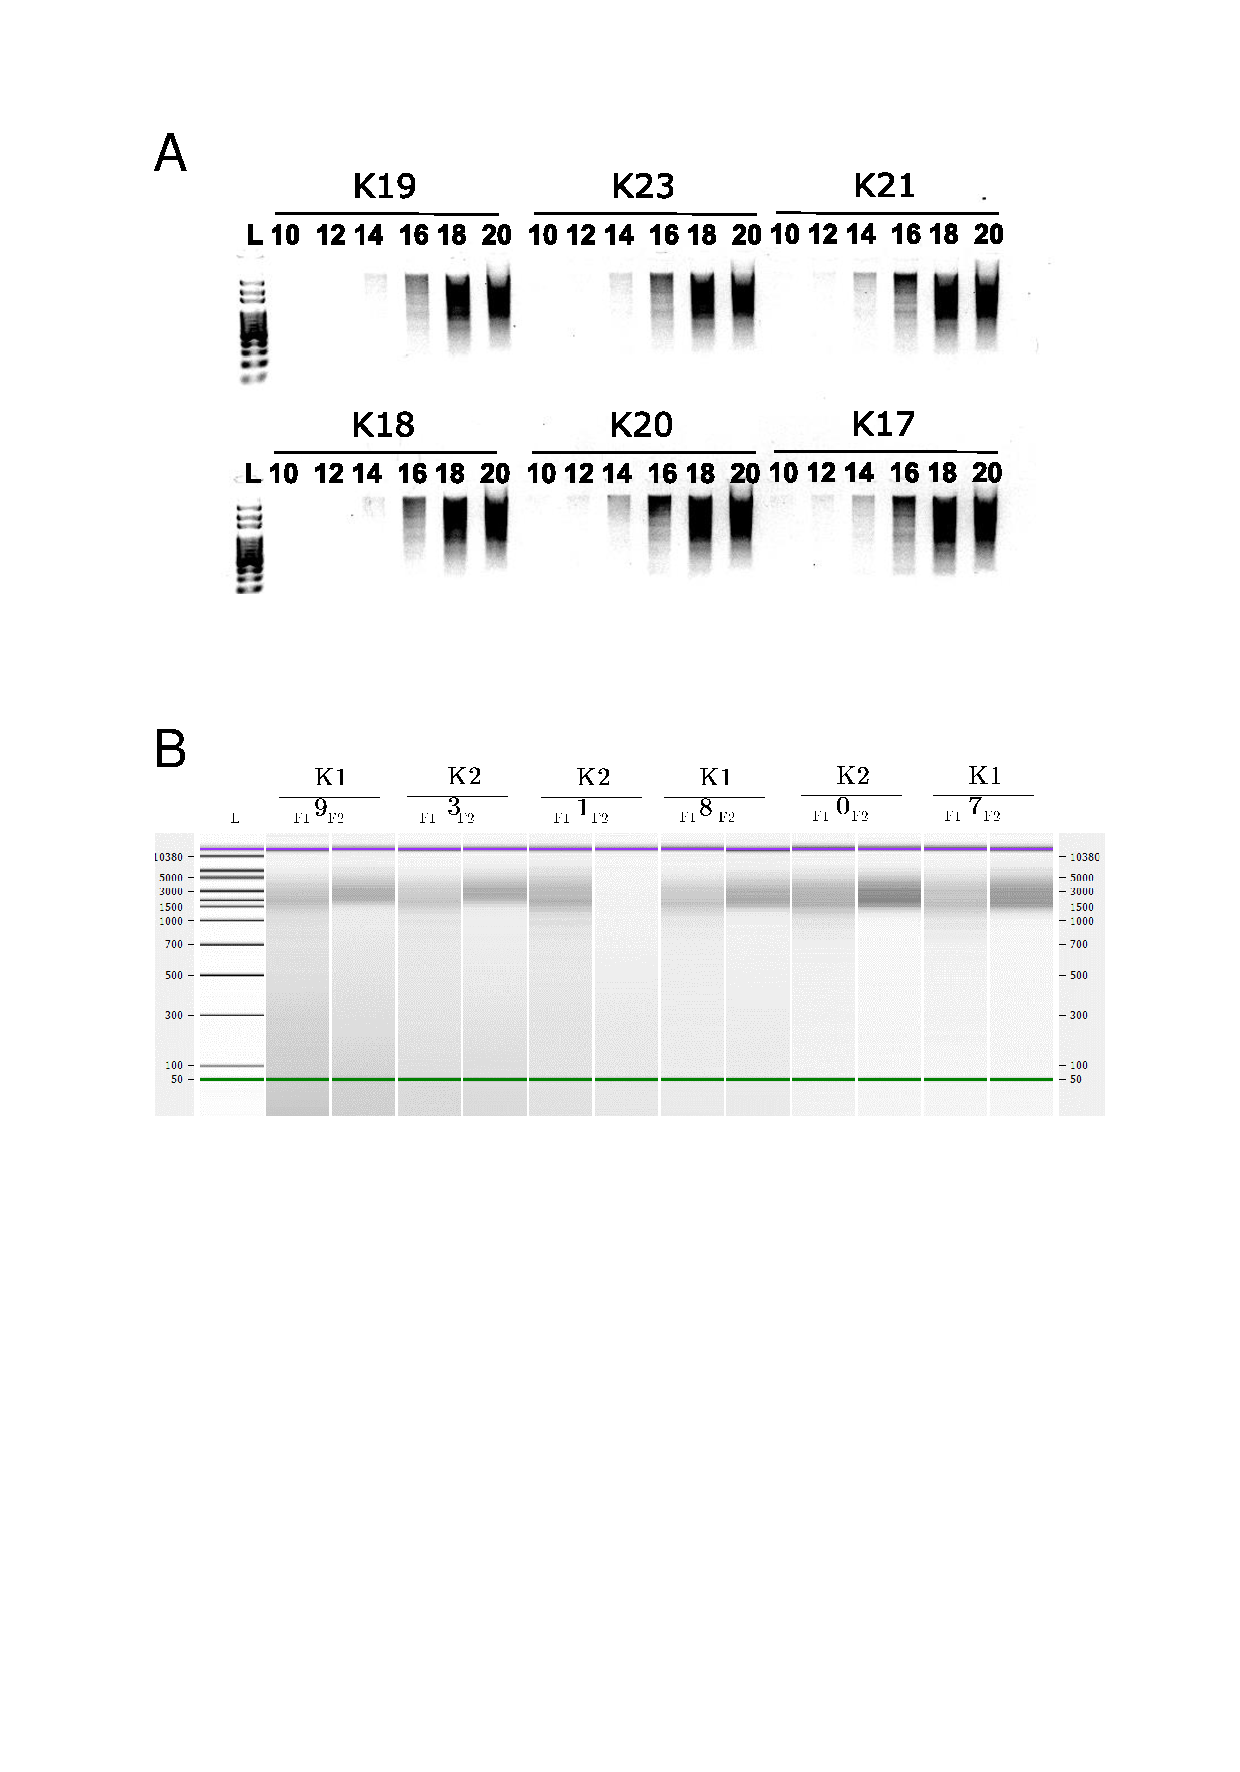
\includegraphics[page=1,trim={0 10cm 0 0cm},clip,scale = 0.75]{Figures/TargetedTranscriptome_ppt.pdf}
	\captionsetup{width=0.95\textwidth}
	\caption[Iso-Seq Targeted Transcriptome - cDNA amplification and purification]%
	{\textbf{The first stage between the targeted and whole transcriptome sequencing is the same with samples typically amplified using 14 cycles followed by enrichment of high molecular weight cDNA in Fraction 2: a)} Like whole transcriptome sequencing, samples were amplified using 14 cycles (Figure \ref{fig:isoseq_whole_pccresults}) whereby cycles below generated insufficient cDNA and cycles above showed signs of over-amplification. The samples shown here (K19, K23, K21, K18, K20, K17) were multiplexed and sequenced in Batch 1 (see Table \ref{tab:mouse_samples_sequenced}. Ladder (L) shown is 100bp DNA ladder. \textbf{B)} Similar to whole transcriptome sequencing, amplified cDNA was further divided into two fractions (denoted here as F1 and F2) and purified with 1X (F1) and 0.4X (F2) AMPure beads. As shown in the Bioanalyzer gel, there was an enrichment of higher-molecular weight cDNA in Fraction 2 compared to Fraction 1 across all the samples (with the exception of Sample K21 with loss of Fraction 2). Green and purple line represent the lower marker at 50bp and the upper marker at 17kb respectively. F1 - Fraction 1 containing cDNA purified with 1X AMPure beads; F2 - Fraction 2 containing cDNA purified with 0.4X AMPure beads.}
	\label{fig:isoseq_targeted_pccresults}
\end{figure}


\begin{figure}[!htp]
	\centering
	\vspace{20pt}
	\includegraphics[page=2,trim={0 8cm 0cm 1cm},clip,scale = 0.75]{Figures/TargetedTranscriptome_ppt.pdf}
	\captionsetup{width=0.95\textwidth}
	\caption[Iso-Seq Targeted Transcriptome - Target Capture and library preparation]%
	{\textbf{Successful target capture and library preparation across all batches, as shown by enrichment of transcripts with specific lengths:} \textbf{A)} and \textbf{c)} are Bioanalyzer electropherogram traces of Batch 1 (n = 6) and Batch 2 (n = 9) respectively after enrichment of cDNA with selective IDT probes ( \cref{section:ch2_targetcapture_explanation}). \textbf{B)}, \textbf{d)} and \textbf{f)} are Bioanalyzer electropherogram traces of Batch 1, 2 and 3 respectively after library preparation (denoted here as "Final", \cref{section:ch2_smrtbelltemplate_explanation}. \textbf{e)} An overlay of Batch 2 after target capture and library preparation. 
	\\
	\\
	As can be seen across all figures, target capture appears to be successful with detected peaks, reflecting enrichment of target transcripts with specific lengths, which differs from the broad peaks that are evident in whole transcriptome sequencing (Figure \ref{fig:isoseq_whole_bioresults}). Library preparation with ligation of SMRT bell templates retained these targeted transcripts with good peak overlay, as seen in figure e). The difference in peak height (i.e. cDNA quantity) between target capture and library preparation is due to a difference in input cDNA concentration when running Bioanalyzer - input cDNA after library preparation was diluted with a 1:5 dilution factor to maximise amount of cDNA available for sequencing, whereas input cDNA after target capture was not diluted.}  
	\label{fig:isoseq_targeted_libresults}
\end{figure}

\begin{figure}[!htp]
	\centering
	\vspace{20pt}
	\includegraphics[page=3,trim={0 18cm 0cm 0cm},clip,scale = 0.75]{Figures/TargetedTranscriptome_ppt.pdf}
	\captionsetup{width=0.95\textwidth}
	\caption[ONT Targeted Transcriptome - Target Capture and library preparation]%
	{\textbf{Successful target capture and ONT library preparation, as shown by enrichment of transcripts with specific lengths:} Shown in \textbf{A)} is the gel snapshot image from the TapeStation Assay of Batch 2 (n = 9) and Batch 3 (n = 9) respectively after enrichment of cDNA with selective IDT probes (\cref{section:ch2_targetcapture_explanation}) and ONT library preparation (\cref{sec: ONTlib_preparation}), and \textbf{B)} is the respective electropherogram of Batch 3. 
	\\
	\\
	Similar to the Bioanalyzer electropherogram from \cref{fig:isoseq_targeted_libresults}, target capture and ONT library preparation appears to be successful with detected peaks, reflecting enrichment of target transcripts with specific lengths. Diluted DNA (1:5 dilution factor) was used for TapeStation Assay to maximise the amount of cDNA available for sequencing. L - Ladder, B2 - Batch 2, B3 - Batch 3. Of note, the ladder used was expired and thus missing the lower green marker. }  
	\label{fig:ONT_targeted_libresults}
\end{figure}


\subsection{ONT Library Preparation and Nanopore Sequencing}
RNA from a subset of mouse samples (n = 2) was prepared for ONT cDNA library preparation and nanopore sequencing using the ONT lab workflow, as detailed and described in \cref{chap:ont_labpipeline}. Briefly, cDNA was similarly prepared from 200ng RNA using the SMARTer PCR cDNA Synthesis Kit (Clontech, UK) (described in \cref{section:ch2_cDNA_synthesis_explanation}), with addition of ERCC standards, followed by PCR amplification of 14 cycles with PrimeSTAR GXL DNA Polymerase (Clontech, UK) (described in \cref{section:ch2_PCR_explanation}). Quantification and size distribution were then determined using Qubit DNA High sensitivity assay (Invitrogen) and Bioanalyzer 2100 (Agilent), and library preparation was proceeded with ONT’s Ligation Sequencing kit (SQK-LSK109) (detailed in \cref{sec: ONTlib_preparation}). Sequencing was then performed on ONT MinION using a FLO-Min106D flow cell (detailed in \cref{sec: ONTlib_sequencing}). 

\subsection{ONT QC and data processing}
QC of raw reads was performed using PycoQC, with subsequent analysis using the ONT bioinformatics pipeline (details are provided in \cref{section:ont_bioinformatics}). Briefly, raw reads were basecalled using \textit{Guppy} (v4.0) and reads with Phred (Q) < 7 filtered out. Primers and ONT adapters were then removed using \textit{Porechop} to generate full-length reads, followed by trimming of polyA tails with \textit{Cutadapt}. Full-length reads were then mapped to the reference mouse genome using \textit{Minimap2} (v2.17) with the following parameters "-ax splice". Owing to the high error rate attributed to ONT sequencing, artifactual noncanonical splice junctions from aligned reads were corrected with \textit{Transcript Clean} and corrected reads were subsequently processed using \textit{TALON} for annotation, quantification and filtering for intrapriming (--maxFracA = 0.5). Novel transcripts were only retained if detected with minimum 2 reads in at least 2 samples. 
 
\begin{figure}[htp]
	\centering
	\includegraphics[page=16,trim={0cm 8cm 0cm 0cm},clip,scale = 0.8]{Figures/ProjectDevelopment_Figures}
	\captionsetup{width=0.95\textwidth,singlelinecheck=off}
	\caption[ONT Bioinformatics Pipeline]%
	{\textbf{ONT Bioinformatics Pipeline.} Shown is a detailed bioinformatics pipeline for processing ONT 1D reads from the targeted sequencing experiments, whereby 20 samples were barcoded and sequenced simultaneously on two flow cells (referred as Batch 2 and Batch 3 of the original Iso-Seq Targeted Transcriptome set). Supplementing \cref{fig:ONT_PacBio_bioinformatics}, raw ONT reads from each flow cell were processed and the demultiplexed into the respective samples, which were then processed independently for collapse and transcript quantification. All the samples from both batches were then merged into one complete dataset, while retaining sample-specific transcript expression. 
	}
	\label{fig:ONT_Targeted_bioinformatics}
\end{figure}

\subsection{Comparison of Iso-Seq and Nanopore datasets}
The Iso-Seq targeted dataset (n = 24 samples) was examined with other datasets using \textit{Gffcompare}; such datasets included transcripts identified from whole transcriptome profiling (n = 12 samples) and ONT-derived transcripts from nanopore targeted sequencing (n = 18 samples). For a fairer comparison, Iso-Seq transcripts from whole transcriptome profiling were re-annotated with \textit{SQANTI3} with no splice junction filtering from short-read RNA-Seq data, and only coverage from the same samples were used for the comparison between the whole and targeted Iso-Seq datasets. Conversely, all processed but unfiltered ONT reads were used for a comprehensive comparison between the two technologies with Iso-Seq derived transcripts as reference.   

\subsection{Transcript annotation and Iso-Seq Quantification}
For a comprehensive characterisation of the AD-associated genes enriched in the mouse transcriptome, the Iso-Seq and ONT datasets were merged using \textit{Gffcompare}. In order to retain both filtered ONT-derived transcripts (minimum 2 reads in at least 2 samples) and ONT-derived transcripts that did not pass through filtering but were also detected using the Iso-Seq platform, a custom python script was written to parse the output from \textit{Gffcompare} to identify Iso-Seq and ONT-derived transcripts with a complete exact match (defined by the class code "="), unique filtered ONT-derived and unqique Iso-Seq-derived transcripts. An output file of the abundance was also generated for each transcript and sample, using the counts either provided from \textit{Cupcake} for Iso-Seq-derived-transcripts, \textit{TALON} for ONT-derived-transcripts or the summation of both for transcripts that were commonly detected in both technologies. The merged dataset was then annotated with \textit{SQANTI3} in combination with mouse reference gene annotations (mouse GENCODE, vm22), FANTOM5 CAGE peaks and \textit{STAR}-aligned RNA-Seq junctions, and were classified as either FSM, ISM, NIC, NNC, antisense, fusion, and intergenic (described in \cref{section: sqanti_annotations}). Transcripts classified as ISM with 3'fragment were assumed to be partial 5'RNA degraded products and discarded. ORFs were predicted using the CPAT program (v3.0.2) using all default parameters and transcripts were predicted as protein-coding if the coding potential score was >0.44 for mouse (CPAT recommended parameters)  

\subsection{Characterisation of AS events and transcript visualisation}
To date, current tools for assessing alternative splicing events were developed for short-read RNA-Seq data and fail to capture the connectivity and complexity of long-read-derived isoforms, particularly in targeted profiling of the transcriptome with deep sequencing coverage. A custom python script was therefore written to accurately assess the occurrence of alternative splicing events based on splice junction coordinates of transcript exons relative to exons of all known GENCODE transcripts (mm10). Common alternative splicing events such as alternative first exons (AF), alternative last exons (AL), alternative 5' splice sites (A5), alternative 3' splice sites (A3), intron retention (IR) and exon skipping were assessed. Furthermore, other regulatory mechanisms such as alternative transcription initiation defined by alternative promoter/TSS, alternative termination likewise defined by alternative TTS, and presence of novel exons were evaluated using this custom script.


Alternative 5' and 3' splice sites were defined as splice sites differing by more than 10bp from the known splice site, and an intron was considered retained if the exon splice site differed by more than 100bp from the known splice site. Isoforms were visualised using UCSC genome browser, and were grouped by their splicing patterns to ease visualisation based on the following rank prioritisation: i) all exons with exact splice junction coordinates to know exons, ii) alternative first exons, iii) contain novel exons upstream of first exon, iv) novel exons downstream of last exon, v) characterised with intron retention, exon skipping and novel exons, vi) IR and ES, vii) novel exons within known exons, viii) IR only, ix) ES only and x) all exons with alternative 5' and 3' sites.

%ISM isoforms were assumed as partial products of longer FSM isoforms, and associated read counts were aggregated.  

\begin{figure}[htp]
	\centering
	\includegraphics[page=5,trim={0.5cm 7cm 0cm 0cm},clip,scale = 0.8]{Figures/TargetedTranscriptome_LabResults}
	\captionsetup{width=0.95\textwidth,singlelinecheck=off}
	\caption[Bioinformatics Pipeline for merging targeted Iso-Seq and ONT datasets]%
	{\textbf{Bioinformatics Pipeline for merging targeted Iso-Seq and ONT datasets}. Shown is a outline of the bioinformatics pipeline for processing Iso-Seq reads and ONT reads 1D reads from the targeted transcriptome profiling of the mouse cortex. 
	}
	\label{fig:Targeted_bioinformatics_pipeline}
\end{figure}

\newpage
\section{Results}
\subsection{Iso-Seq Run performance and sequencing metrics}
Following Iso-Seq library preparation and SMRT sequencing, a total of XXGb (s.d = XXGb) were obtained (Table \ref{tab:targeted_mouse_run_output}). Of note, 6 samples were first trialled and multiplexed in Batch 1 to determine the yield output and coverage depth - PacBio recommends starting with 4 - 8 samples for multiplexing. Having noticed that an average yield output (24Gb) with a high off-target sequencing, implicating saturation of target genes with 6 samples, the number was increased to 9 samples in Batch 2 and Batch 3. Despite more samples, the sequencing run for Batch 2 and 3, performed by Exeter's Seqeuncing Service, had a poor loading rate (38.1\% P1 of Batch 3 vs 71\% of Batch 1) and low subsequent yield. The samples were also potentially degraded after having been stored in -20\textdegree C for over 6 months due to Covid-19 lockdown. 

The yield difference between the first and last two batches was evident in the number of CCS reads (total = 996K; Batch 1 = 469K, Batch 2 = 306K, Batch 3 = 2221K Figure \ref{fig:isoseq_targeted_run_output}a) and FLNC reads (total = 930K; Batch 1 = 399K, Batch 2 = 275K, Batch 3 = 256K, Figure \ref{fig:isoseq_targeted_run_output}a) generated, after applying the bioinformatics Iso-Seq pipeline (same as the whole transcriptome approach with the exception of removing barcodes rather than general primers). However, calculation of the on-target rate suggested that while Batch 2 and 3 had lower output yield, the coverage of target genes was significantly greater than Batch 1 due to the increased sample size (mean rate in Batch 1 = 34.5\%; mean rate in Batch 2 = 46.2\%; mean rate in Batch 3: 42.9\%, Figure \ref{fig:isoseq_targeted_rate}). The on-target rate is defined as the proportion of mapped transcripts with sequences overlapping at least one target probe. 
%Off-target 

In addition to batch variability, the number of full-length transcripts obtained per sample varied within each batch (Figure \ref{fig:isoseq_targeted_run_output}b). This variability was not associated with RIN (corr = 0.147, P = 0.492, Spearman's rank) and is unlikely to be due to library preparation, given that samples were pooled in equal molarity during target capture. However, there was no significant difference in the number of full-length transcripts between WT and TG across the batched runs (Wilcoxon rank sum test, W = 73, P = 0.977, Figure \ref{fig:isoseq_targeted_run_output}c). 


\begin{table}[]
	\captionsetup{width=1.0\textwidth}
	\caption[Run Yield Output from Targeted Transcriptome Iso-Seq of Tg4510]%
	{Iso-Seq run yield for each batch of Tg4510 mouse samples sequenced using targeted transcriptome approach}
	\label{tab:targeted_mouse_run_output}
	\centering
	\begin{tabularx}{\textwidth}{cccccccccc}
		\toprule
		\multirow{3}{*}{Sample} &
		\multirow{3}{*}{\begin{tabular}[c]{@{}c@{}}Total \\ Bases\\ (GB)\end{tabular}} &
		\multirow{3}{*}{\begin{tabular}[c]{@{}c@{}}Polymerase\\  Reads\end{tabular}} &
		\multicolumn{4}{c}{Read  Length (kB)} &
		\multicolumn{3}{c}{Productivity} \\ \cmidrule(l){4-10} 
		&&&
		\multicolumn{2}{c}{Polymerase} &
		\multicolumn{2}{c}{Subread} &
		\multirow{2}{*}{P0} &
		\multirow{2}{*}{P1} &
		\multirow{2}{*}{P2} \\
		&&&
		Mean & N50 & Mean & N50 &&&
		\\ \midrule
		Batch 1 & 24.2 & 712250 & 34.0 & 70.5 &	1.4 & 1.85 &
		\begin{tabular}[c]{@{}c@{}}4.62\% \\ (46613)\end{tabular} &
		\begin{tabular}[c]{@{}c@{}}71.58\% \\ (722026)\end{tabular} &
		\begin{tabular}[c]{@{}c@{}}24.76\% \\ (249707)\end{tabular} \\
		Batch 2 &
		&&&&&&&
		&
		\\
		Batch 3 &	19.3 &	383292 &	50.5 &	100 &	1.6 &
		2.02 &
		\begin{tabular}[c]{@{}c@{}}18.68\% \\ (189549)\end{tabular} &
		\begin{tabular}[c]{@{}c@{}}38.11\% \\ (386743)\end{tabular} &
		\begin{tabular}[c]{@{}c@{}}43.56\% \\ (442054)\end{tabular} \\ \bottomrule
	\end{tabularx}

	\vspace{1cm}
	\centering
	\begin{tabularx}{\textwidth}{cccccccc}
		\hline
		\multirow{3}{*}{Sample} & \multicolumn{4}{c}{Control}  & \multirow{3}{*}{\begin{tabular}[c]{@{}c@{}}Local\\ Base\\ Rate\end{tabular}} & \multicolumn{2}{c}{Template} \\ \cline{2-5} \cline{7-8} 
		&
		\multirow{2}{*}{\begin{tabular}[c]{@{}c@{}}Total\\  Reads\end{tabular}} &
		\multirow{2}{*}{\begin{tabular}[c]{@{}c@{}}Read \\  Length Mean\end{tabular}} &
		\multicolumn{2}{c}{Concordance} &
		&
		\multirow{2}{*}{\begin{tabular}[c]{@{}c@{}}Adapter\\ Dimer (0-10bp)\end{tabular}} &
		\multirow{2}{*}{\begin{tabular}[c]{@{}c@{}}Short Insert\\ (11- 100bp)\end{tabular}} \\
		&       &        & Mean & Mode &                                                                              &               &              \\ \hline
		Batch 1                 & 9,690 & 31,505 & 0.84 & 0.87 & 2.31                                                                         & 0             & 0            \\
		Batch 2                 &       &        &      &      &                                                                              &               &              \\
		Batch 3                 & 3,440 & 52,533 & 0.85 & 0.87 & 2.86                                                                         & 0             & 0            \\ \hline
	\end{tabularx}
\end{table}


\begin{figure}[!htp]
	\begin{center}
		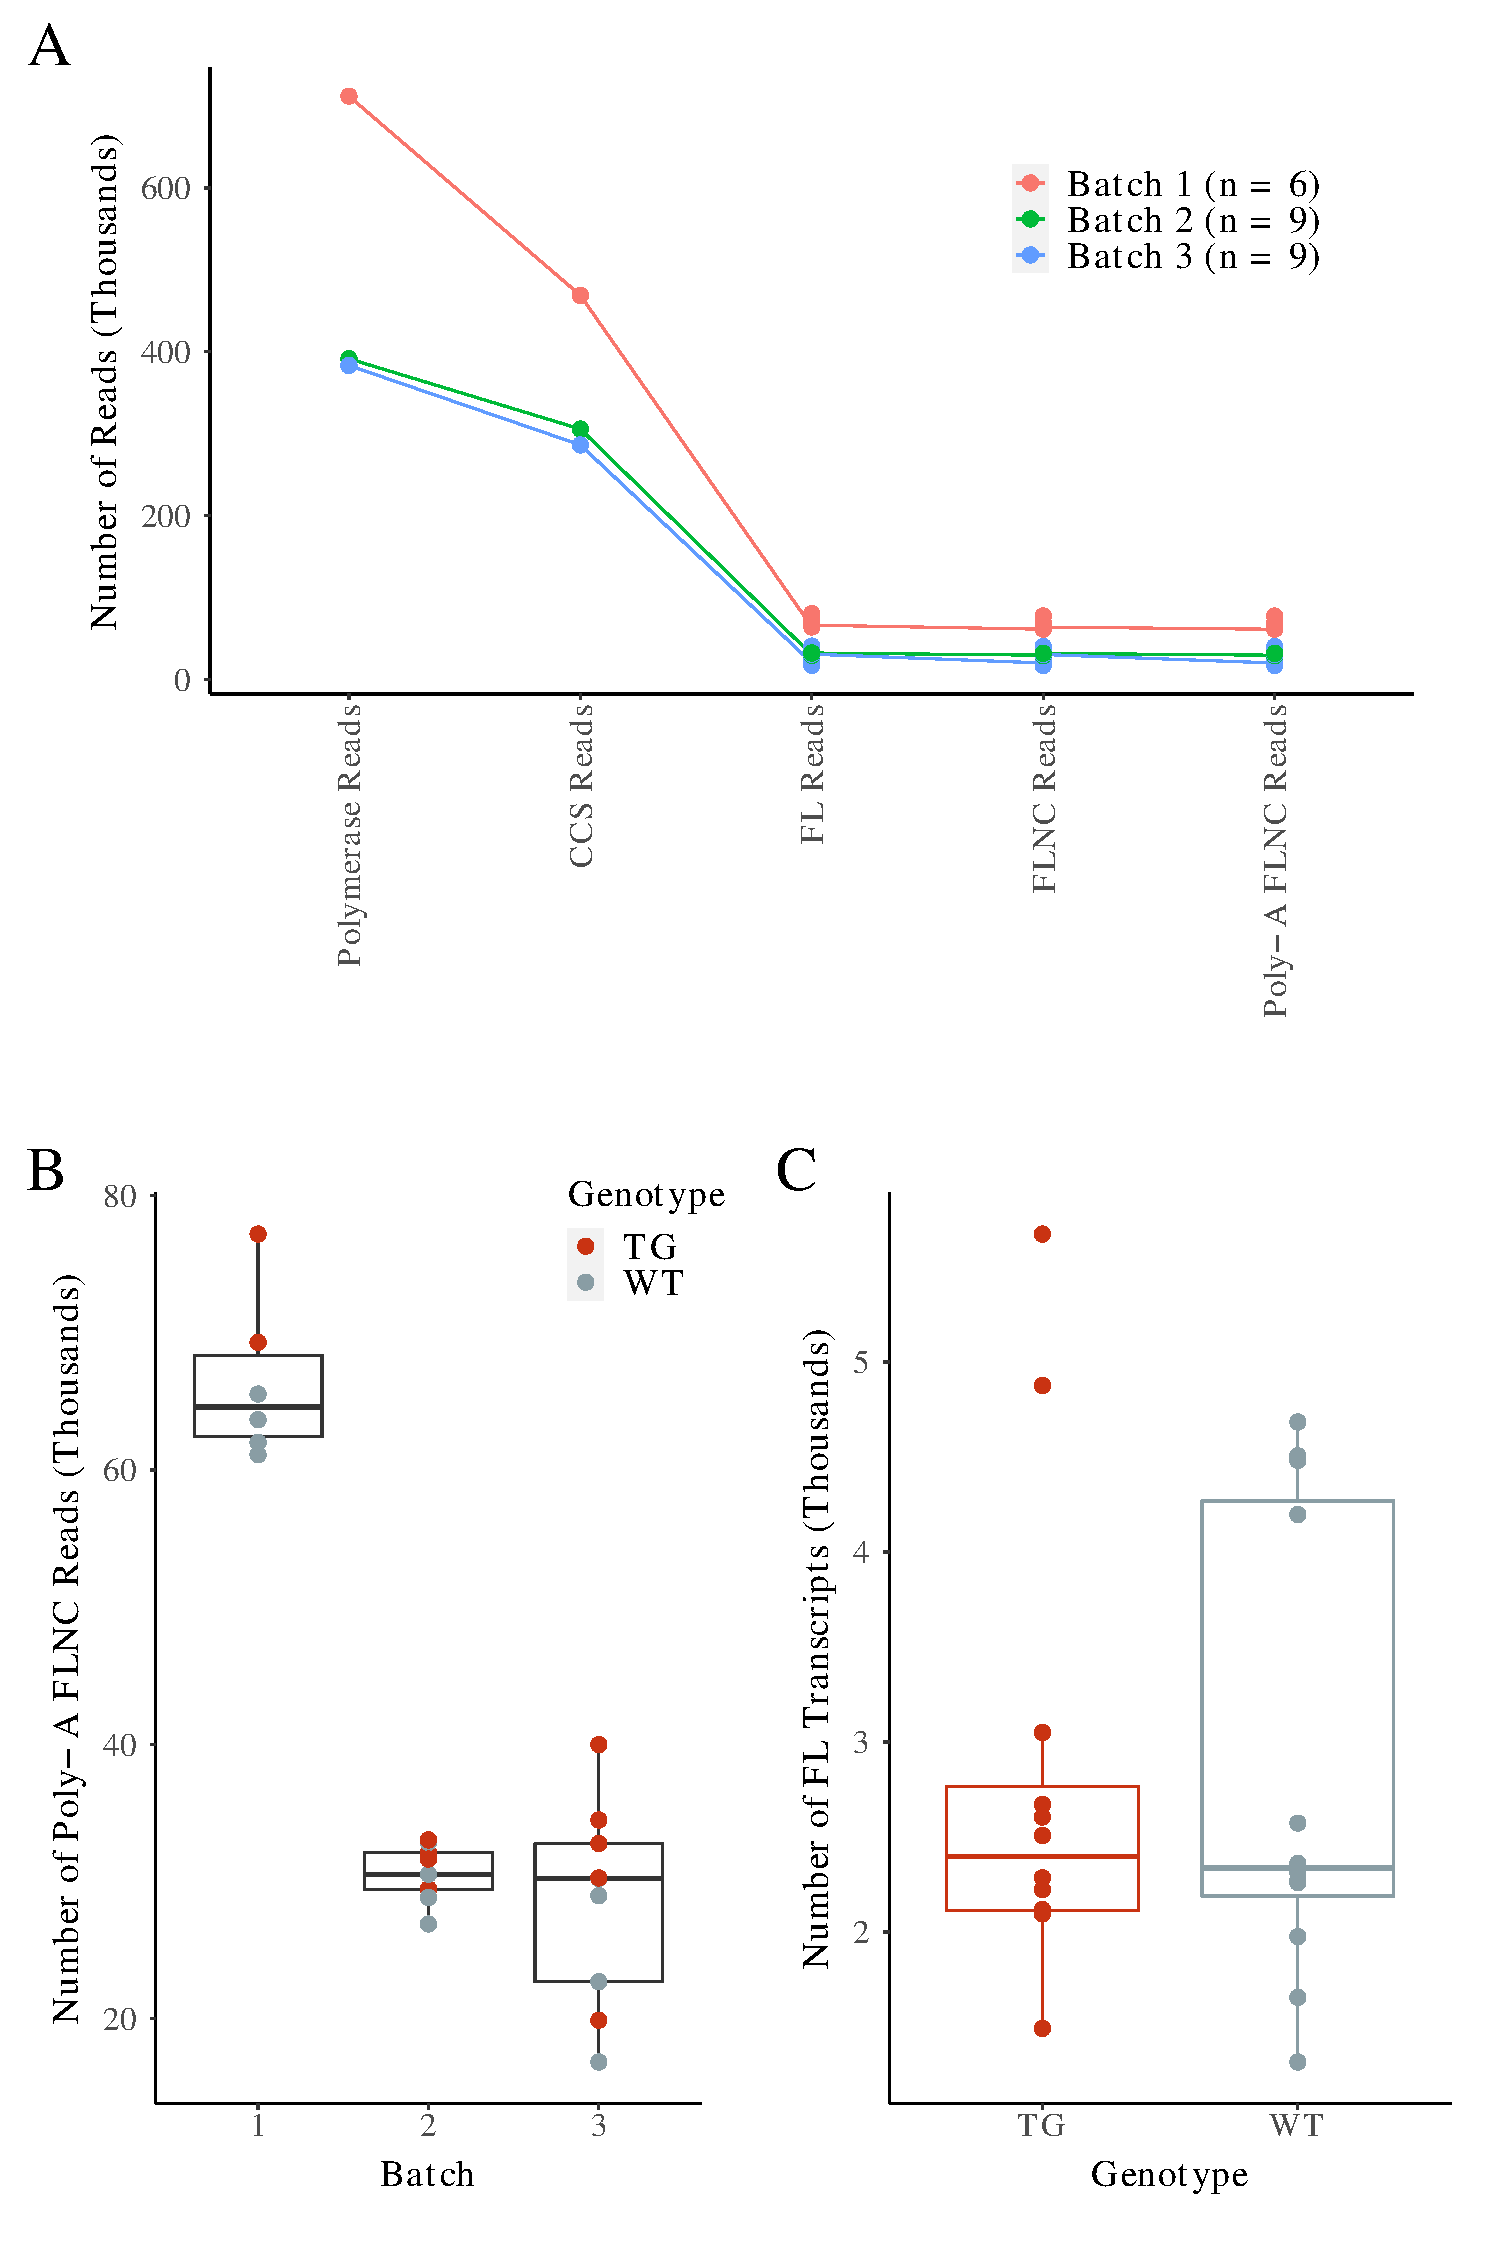
\includegraphics[page=1,trim={0 1cm 0 0},clip,scale = 0.55]{Figures/TargetedTranscriptome.pdf}
	\end{center}
	\captionsetup{width=0.95\textwidth}
	\caption[Targeted Transcriptome Iso-seq run performance]%
	{\textbf{Despite batch variability in targeted transcriptome sequencing, no difference in the number of full-length transcripts was observed between wildtype and transgenic mice}. \textbf{A)} Samples (n = 24) were multiplexed and sequenced in three runs (Batch 1, 2 and 3) with varied performance, as indicated by the number of polymerase reads through to poly-A FLNC reads. In the bioinformatics pipeline, the samples were demultiplexed and individually processed after generation of CCS reads from each run. \textbf{B)} Sample variability within each batch was observed from the number of poly-A FLNC reads generated. However, \textbf{c)} no statistical difference was observed in the overall number of full-length transcripts detected between wild-type and transgenic. Full-length transcripts were collapsed from poly-A FLNC reads in Iso-Seq Cluster. CCS - Circular Consensus Sequence, FLNC - Full-Length Non-Concatemer, FL - Full-Length, WT - Wild-type, TG - Transgenic}
	\label{fig:isoseq_targeted_run_output}
\end{figure}

\begin{figure}[!htp]
	\begin{center}
		\includegraphics[page=2,trim={0 25cm 0 0},clip,scale = 0.55]{Figures/TargetedTranscriptome.pdf}
	\end{center}
	\captionsetup{width=0.95\textwidth}
	\caption[On-Target rate in Transcriptome Iso-Seq runs]%
	{\textbf{Coverage of target genes was greater in Batch 2 and 3 than Batch 1 due to more samples multiplexed and sequenced}. Samples (n = 24) were multiplexed and sequenced in three runs (Batch 1 = 6 samples, Batch 2 = 9 samples, Batch 3 = 9 samples). Despite lower run yield output (\ref{tab:targeted_mouse_run_output}), Batch 2 and Batch 3 had a higher on-target rate, which refers to the proportion full-length transcripts associated with target genes. A difference in the on-target rate between wild-type and transgenic samples was observed in Batch 1, which is a likely reflection of the sample variability in sequencing (Figure \ref{fig:isoseq_targeted_run_output}b). WT - Wild-type, TG - Transgenic}
	\label{fig:isoseq_targeted_rate}
\end{figure}


\subsection{ONT Run performance and sequencing metrics}
Following library preparation and nanopore sequencing on a subset of samples, a total of 28.54M reads (39.68Gb) were generated across two flow cells and a total of 22.8M (80\%) reads were successfully basecalled using \textit{Guppy} (\cref{tab:ont_targetedrun_output}). Despite similar amount of loading onto the flow cell (Batch 2: 540ng, Batch 3: 500ng), there was a large yield difference in the number of basecalled reads between the two batches with Batch 3 generating significantly more reads (Batch 2: 12.3M and Batch 3: 16.3M), and after filtering for read quality (Phred Score > Q7, referring to a read accuracy > 80\%) of which the majority reads passed (Batch 2: 9.68 (78.8\%); Batch 3: 13.13M (99.3\%) (\cref{fig:ONT_targeted_run_output}\textbf{a}). 

Similar to Iso-Seq Targeted Transcriptome run performance, the number of filtered reads obtained per sample varied within each batch (\cref{fig:ONT_targeted_run_output}\textbf{B}), with more reads generated in the transgenic mice in both Batches 2 and 3 (\cref{fig:ONT_targeted_run_output}\textbf{c}, Batch 2: Wilcoxon rank sum test, W = 18, P = 0.063; Batch 3: Wilcoxon rank sum test, W = 17, P = 0.11). This variability was not associated with RIN (corr = -0.267, P = 0.284, Spearman's rank) or barcode (corr = -0.058, P = 0.819, Spearman's rank), but simply a reflection of more transgenic mice sequenced (Batch 2: WT = 4, TG = 5 samples; Batch 3: WT = 4, TG = 5 samples). The difference in number of WT and TG mice in Batches 2 and 3 would have been compensated in Iso-Seq with Batch 1, where there is more WT mice; however, Batch 1 was not sequenced using ONT due to the lack of remaining cDNA. Of note, the difference in the number of reads between TG and WT, while different, was not statistically significant at the 5\% level (Wilcoxon rank sum test, W = 59, P = 0.10, \cref{fig:ONT_targeted_run_output}\textbf{d}).
  
While the throughput was comparable between Iso-Seq and ONT nanopore sequencing for the targeted transcriptome profiling (Iso-Seq: 19.3 - 24.2Gb, ONT: 16.9 - 22.8Gb), ONT nanopore sequencing generated significantly more (1D) reads (12.3M - 16.3M) than the polymerase reads from Iso-Seq (0.3M - 0.7M), which is limited by the number of wells available for sequencing (1M ZMWs), and subsequently 20X the number of full-length reads per sample (Iso-Seq mean PolyA-FLNC reads = 38.7K, range = 16.8K - 77.2K; ONT mean basecalled, filtered reads = 918K, range = 667K - 1.32M). This significant difference in read but comparable yield output is due to the multiple sequencing of the same insert in Iso-Seq with the generation of CCS reads, whereas each insert is only sequenced once in ONT nanopore. This significantly higher yield is therefore achieved at the expense of read accuracy, whereby the average read accuracy in ONT nanopore is 90\% (mean Phred Quality = 10; \cref{tab:ont_targetedrun_output)}, \cref{fig:ont_targetedlengthquality}\textbf{a,b}). Of note, the on-target rate observed in both Iso-Seq and ONT nanopore sequencing was similar at $\tilde{50\%}$ (\cref{fig:isoseq_targeted_rate,fig:ont_targeted_rate}), indicating that more samples could have been sequenced.  

\begin{figure}[htp]
	\begin{center}
		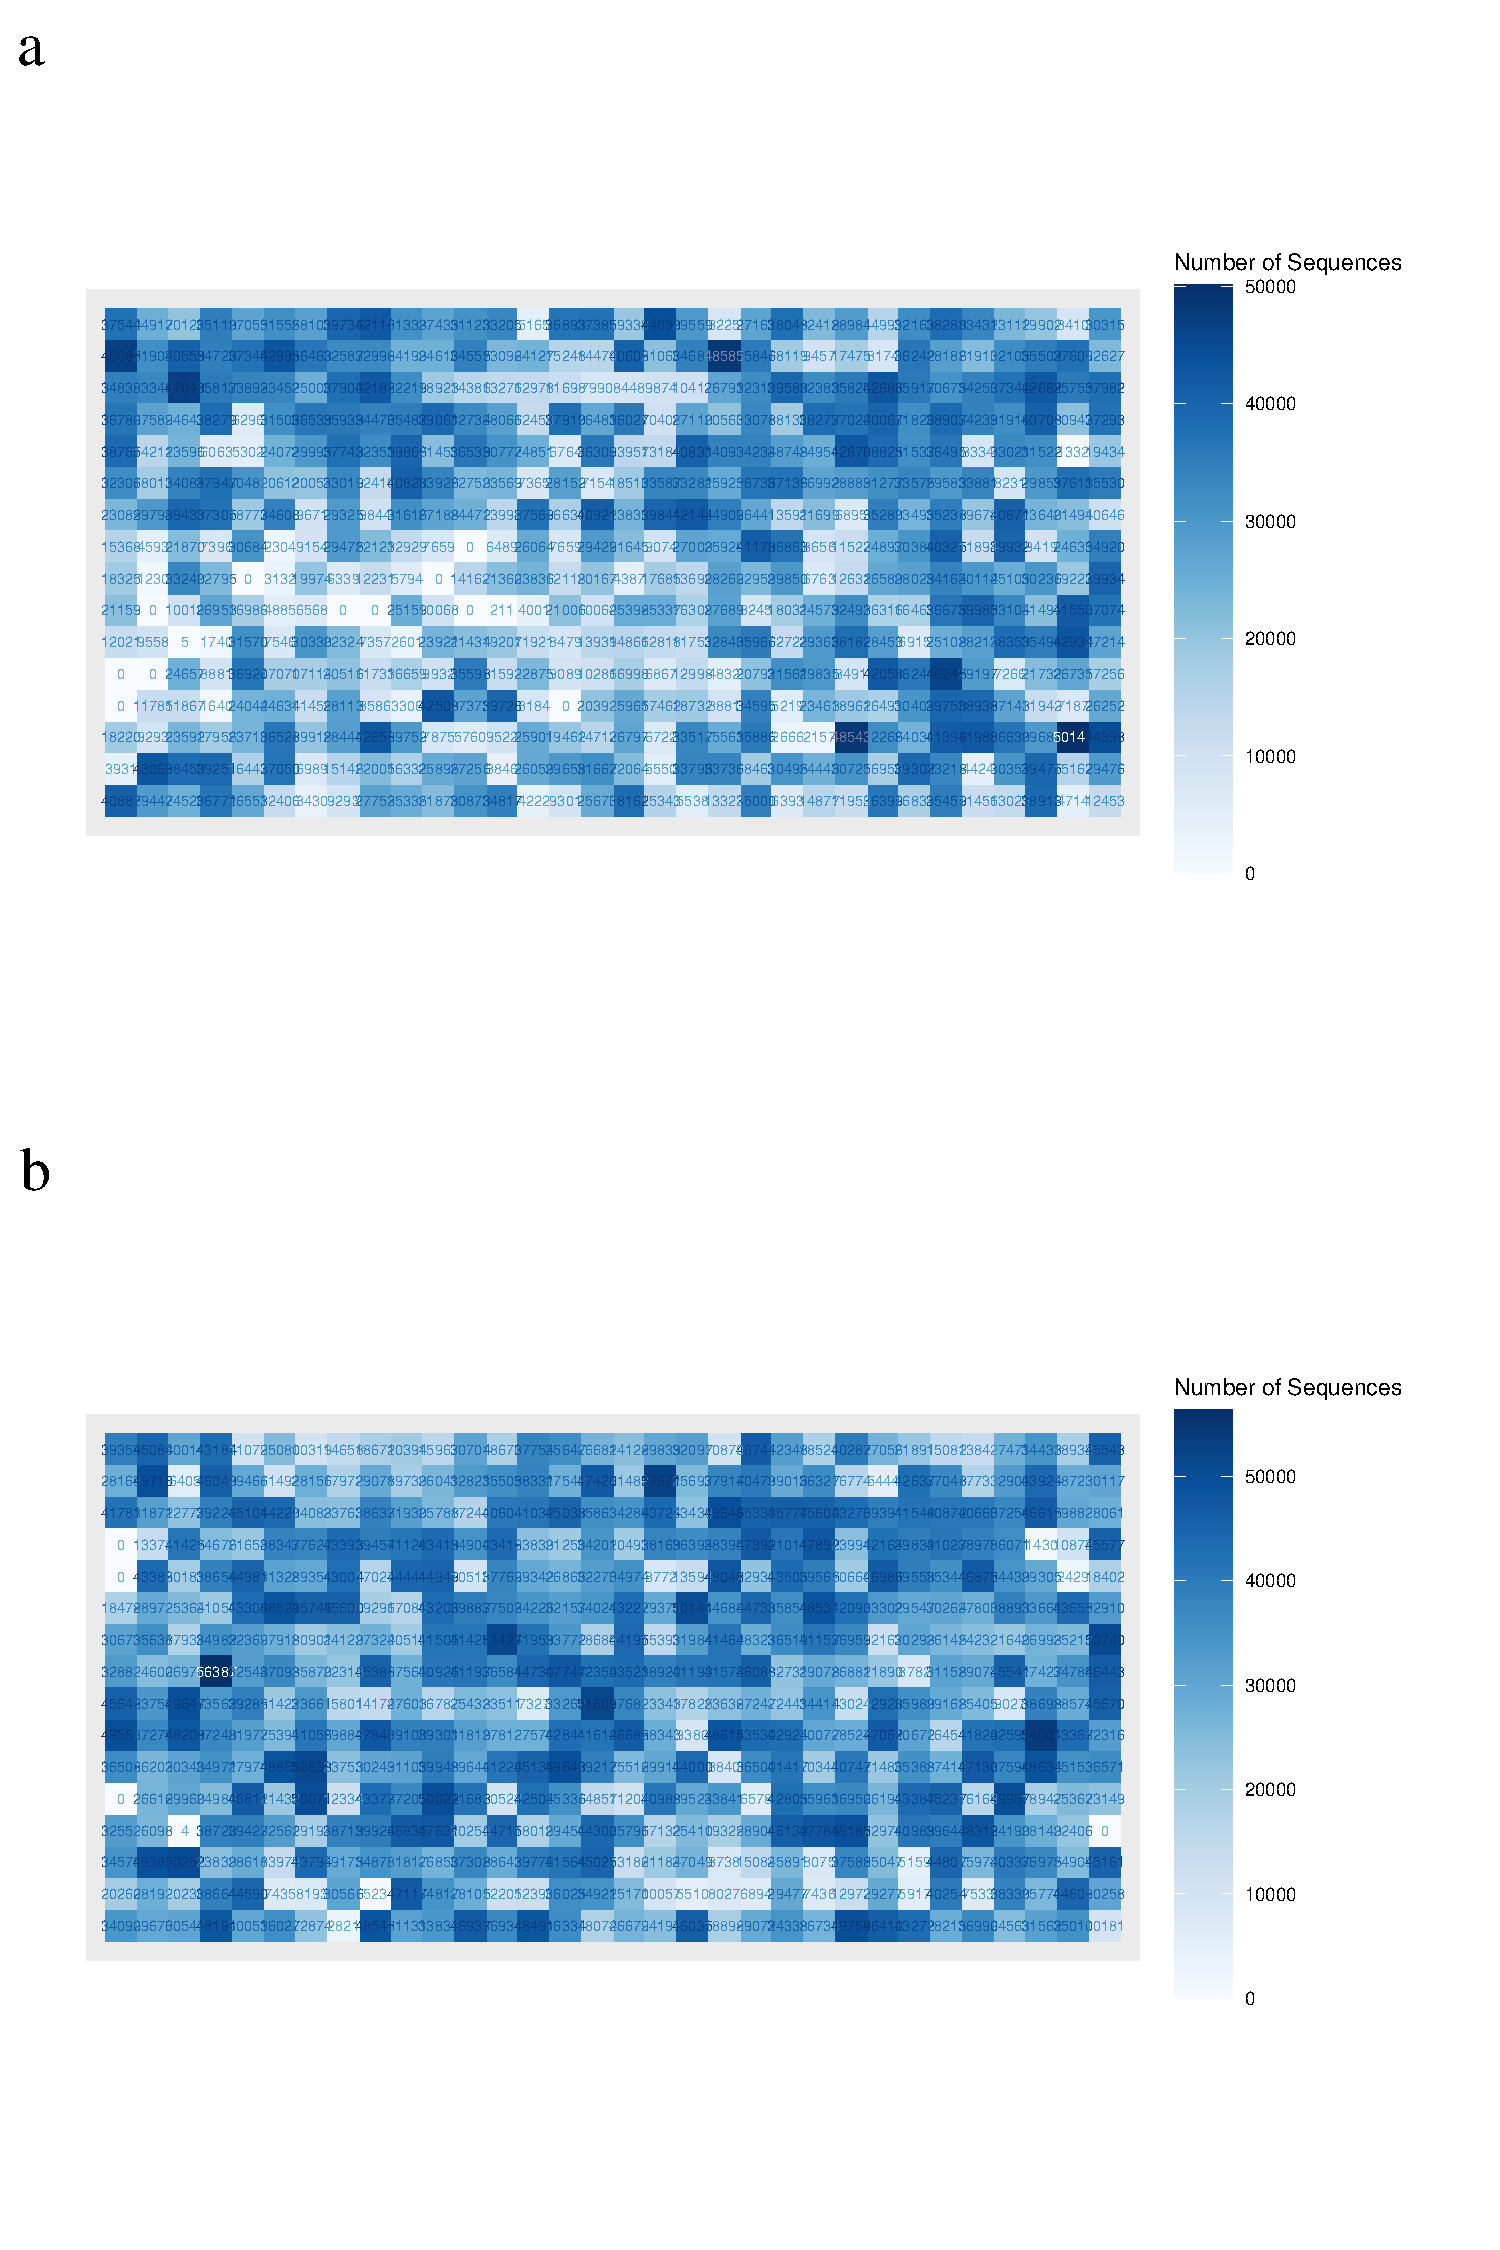
\includegraphics[page=1,trim={0 4cm 0 0},scale = 0.45]{Figures/ONTTargetedTranscriptome.pdf}
	\end{center}
	\captionsetup{width=0.95\textwidth}
	\caption[ONT Sequence Channel Activity from Whole Transcriptome Sequencing ]%
	{\textbf{Sequencing channel activity plot from nanopore sequencing}. Heatmap representation of channel productivity spatially for \textbf{A)} Batch2 (10.1Gb) and \textbf{B)} Batch 3 (3.68Gb) as DNA is translocated through the pore and signal is collected. A contrast of activity can be seen between the two batches, with a number of inactive channels (white box) in Batch 2, and of the channels that are active, fewer DNA molecules are translocated and read.}
	\label{fig:ont_targetedseq_channel}
\end{figure}

%% Qus: Wsa there reflushing?
\begin{figure}[htp]
	\begin{center}
		\includegraphics[page=2,,trim={0 0cm 0cm 10cm},clip, scale = 0.45]{Figures/ONTTargetedTranscriptome.pdf}
	\end{center}
	\captionsetup{width=0.95\textwidth}
	\caption[ONT run performance over time from Whole Transcriptome Sequencing ]%
	{\textbf{Temporal run performance from nanopore sequencing}. Shown is the \textbf{A)} number of basses generated per hour over the course of the sequencing run from Batch 2 and from \textbf{B)} Batch 3, and \textbf{c)} cumulative reads generated from Batch2 and from \textbf{d)} Batch3. The reads are classified as "pass" (dark blue) if QV > 7 and "fail" (light blue) if QV < 7. Gb - Gigabases}
	\label{fig:ont_targetedtime_performance}
\end{figure}


\begin{figure}[!htp]
	\centering
	\includegraphics[page=4,trim={0 0 0 0},clip,scale = 0.55]{Figures/ONTTargetedTranscriptome.pdf}
	\captionsetup{width=0.95\textwidth}
	\caption[ONT Targeted Transcriptome run performance]%
	{\textbf{Significantly more reads were generated in Batch 3 and for transgenic mice in ONT nanopore sequencing}. \textbf{A)} A subset of samples (n = 19) were multiplexed and sequenced in two runs (Batches 2 and 3) with varied performance, as indicated by the number of sequenced reads through to reads demultiplexed per sample. \textbf{B)} Sample variability within each batch not correlated by barcode sequence. \textbf{c)} A reflection of the yield output and sequencing of more transgenic mice, there were more significantly reads generated for transgenic mice individually and \textbf{d)} and across both batches. WT - Wild-type, TG - Transgenic }
	\label{fig:ONT_targeted_run_output}
\end{figure}

\vspace{1cm}
\begin{table}[ht]
	\captionsetup{justification=raggedright,width=0.95\textwidth}
	\caption[Run Yield Output from Targeted Transcriptome Nanopore Sequencing of Tg4510]%
	{\textbf{Comparable run performance and yield output from Targeted Nanopore sequencing of Tg4510}. Two of three batches prepared for targeted transcriptome profiling were also sequenced on ONT MinION on two separate flow cells over 48hours (Batch 2: WT = 4, TG = 5 samples; Batch 3: WT = 4, TG = 5 samples). The number of total reads basecalled was comparable to the targeted sequencing yield with the Iso-Seq approach (\cref{fig:isoseq_targeted_run_output}). Basecalled reads were filtered on quality score with a QV threshold of 7. N50 refers to the sequence length at which 50\% of reads are sized at or over. Gb - Gigabases. Med - Median}
	\label{tab:ont_targetedrun_output}
	\centering
	\begin{tabularx}{0.95\textwidth}{@{}ccccc@{}}
		\toprule
		\multirow{2}{*}{Sample} & \multicolumn{2}{c}{All Reads}      & \multirow{2}{*}{Active channels} & \multirow{2}{*}{Run Duration} \\ \cmidrule(lr){2-3}
		& Total Bases (Gb) & Number of Reads &                                  &                               \\ \midrule
		Batch 2                     & 16.9             & 12,274,792       & 479                              & 48hours                       \\
		Batch 3                     & 22.8             & 16,274,909       & 425                              & 48hours                       \\ \bottomrule
	\end{tabularx}
	\vspace{1cm}

	\begin{tabularx}{0.95\textwidth}{@{}ccccccccc@{}}
		\toprule
		\multirow{2}{*}{Sample} & \multirow{2}{*}{\begin{tabular}[c]{@{}c@{}}Total Bases\\ (Gb)\end{tabular}} & \multirow{2}{*}{\begin{tabular}[c]{@{}c@{}}Number of\\  Reads\end{tabular}} & \multicolumn{4}{c}{Read Length (bp)} & \multicolumn{2}{c}{Read Quality} \\ \cmidrule(l){4-9} 
		&                                                     &                                                                             & Med  & Mean & N50  & Longest Read & Med           & Mean          \\ \midrule
		Batch 2                     & 14.2                                                                        & \begin{tabular}[c]{@{}c@{}}9,675,186 \\ (78.8\%)\end{tabular}               & XXX   & 1478 & 1779 & 19081        & XXX              & 10.2           \\
		Batch 3                     & 19.41                                                                         & \begin{tabular}[c]{@{}c@{}}13,129,731\\  (80.7\%)\end{tabular}               & XXX    & 1468 & 1813 & 20476        & XXX             & 9.9          \\ \bottomrule
	\end{tabularx}
\end{table}


\begin{figure}[ht]
	\centering
	\includegraphics[page=5,trim={0 27cm 0 0cm},clip,scale = 0.55]{Figures/ONTTargetedTranscriptome.pdf}
	\captionsetup{width=0.95\textwidth}
	\caption[On-Target rate in ONT nanopore runs]%
	{\textbf{Comparable on-target rate in ONT nanopore sequencing to Iso-Seq with a 40-50\% on target rate}. Samples (n = 18) were multiplexed and sequenced in two runs (Batch 2 = 9 samples, Batch 3 = 9 samples). The on-target rate, was similar to that observed in Iso-Seq targeted sequencing (\cref{fig:isoseq_targeted_rate}). A difference in the on-target rate between wild-type and transgenic samples was observed in both batches, a likely reflection of the sample variability in sequencing (\cref{fig:ONT_targeted_run_output}\textbf{c,d}). WT - Wild-type, TG - Transgenic}
	\label{fig:ont_targeted_rate}
\end{figure}

\begin{figure}[htp]
	\begin{center}
		\includegraphics[page=3,trim={0 0cm 0cm 10cm},clip, scale = 0.45]{Figures/ONTTargetedTranscriptome.pdf}
	\end{center}
	\captionsetup{width=0.95\textwidth}
	\caption[ONT read length and quality from Whole Transcriptome Sequencing ]%
	{\textbf{Length and quality distribution of ONT basecalled reads}. Shown are histograms of the number of sequenced reads against \textbf{A)} mean read quality score of Batch 2, \textbf{B)} mean read quality score of Batch 3, and against \textbf{c)} length of Batch 2 and of \textbf{d)} Batch 3. The distribution has been shaded for reads that have passed or failed the quality filter (Q-score threshold of 7). N50 refers to the sequence length at which 50\% of reads are sized at or over. }
	\label{fig:ont_targetedlengthquality}
\end{figure}

\clearpage
\subsection{Iso-Seq Targeted approach detects many more novel transcripts than whole transcriptome profiling}
% Number of Iso-Seq transcripts
After filtering for technical artefacts (563 (1.69\%) isoforms were removed due to intra-priming, 314 (0.94\%) isoforms were removed due to RT switching, 1,267 (3.80\%) were removed due to likely partial degradation), a total of 4,780 isoforms were detected across 20 AD-associated target genes across all the samples (n = 24). Of these isoforms, an overwhelming majority were novel (n = 4601, 96.2\%) with no RNA-Seq support (n = 24 samples, total number of uniquely mapped reads = 360 million) at the junction (n = 4,033, 84.4\%). This is likely to be reflection of the low coverage of RNA-Seq reads per sample (mean number of uniquely mapped reads = 15 million) to comprehensively span these novel junctions, rather than an indication of the invalidity of these isoforms given the stringent processing of the Iso-Seq bioinformatics pipeline. 

We next wanted to compare the isoform diversity and sequencing coverage of the panel of AD-associated genes captured using the targeted and whole transcriptome approach. As expected, enrichment and selective sequencing of the target genes detected many more transcripts that were not detected in the whole transcriptome approach, the majority of which were novel (NIC: XX, XX\%; NNC: XX, XX\%). Further examination of these transcripts unique to the targeted approach revealed them to be more lowly-expressed than the transcripts detected from both sequencing approaches, highlighting the greater sensitivity of the targeted approach in detecting the novel, rarer transcripts. 

Conversely with a target rate of \textasciitilde{XX\%}, the targeted sequencing experiments detected many isoforms associated with non-target genes, which were found to be more highly expressed than the isoforms of non-target genes that were uniquely detected in the whole transcriptome approach. This indicates that the off-target genes from the targeted transcriptome are the most abundance rather than based on similar sequence homology to garget genes. 

Intriguingly, the whole transcriptome approach detected isoforms associated with all the target genes with the exception of \textit{Trpa1}, which is the least expressed in the mouse cortex and was only detected in the targeted approach.  Given that we have previously showed that our whole transcriptome Iso-Seq sequencing datasets (n = 12 samples) was close to saturation, we do not anticipate that we would detect \textit{Trpa1} with more samples. This suggests that our sequencing coverage at a total XX Iso-Seq reads were capped at detecting genes above XXTPM.   

\begin{figure}[!htp]
	\begin{center}
		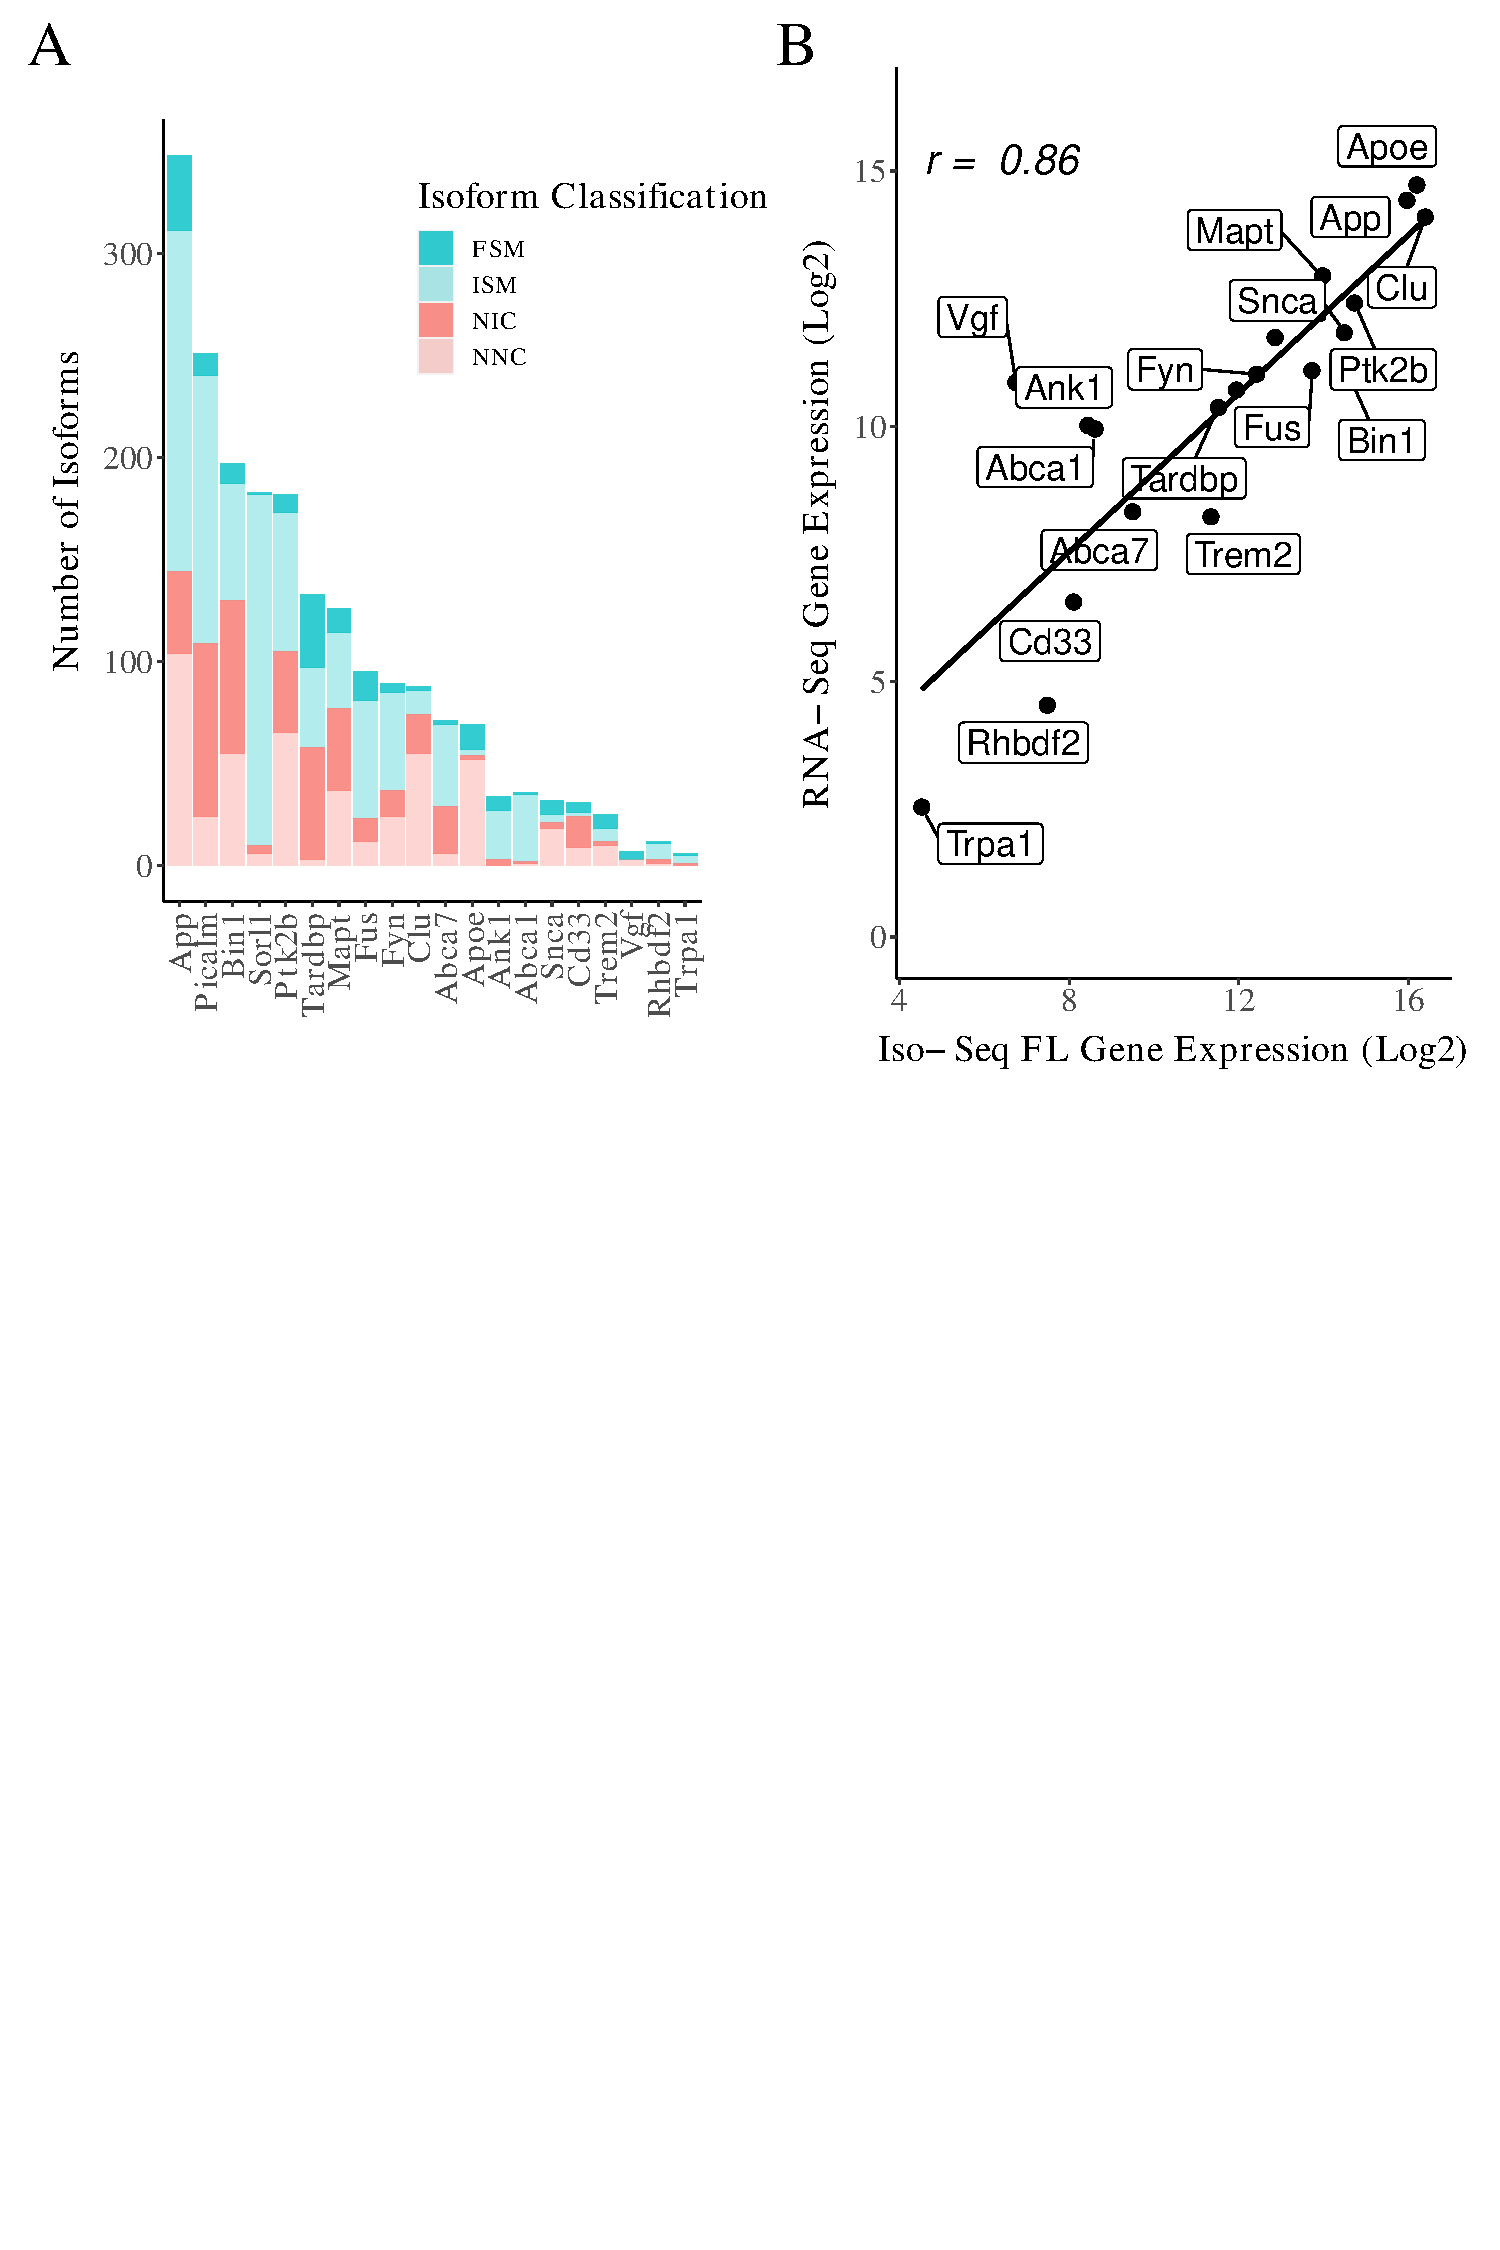
\includegraphics[page=1,trim={0 20cm 0 0cm},clip,scale = 0.60]{Figures/ONTvsIsoSeq.pdf}
	\end{center}
	\captionsetup{width=0.95\textwidth}
	\caption[Wide isoform diversity in AD-associated genes from Targeted Sequencing in mouse cortex]%
	{\textbf{Wide isoform diversity observed in AD-associated genes with many novel isoforms detected}. \textbf{A)} Shown is the number of isoforms detected per target gene from the Iso-Seq targeted dataset, classified by novel and known, after sequential processing and filtering in the bioinformatics Iso-Seq pipeline. Novel isoforms refer to isoforms that are not known in current existing annotations. \textbf{B)} A strong correlation was observed between Iso-Seq and RNA-Seq gene expression. Iso-Seq gene expression was determined from the summation of full-length read counts of associated transcripts, whereas RNA-Seq gene expression was deduced from the normalised \textit{DESeq} counts of aligned RNA-Seq reads to reference genome\cite{Castanho2020}.}
	\label{fig:isoseq_targeted_finalnumberiso}
\end{figure}


\begin{figure}[!htp]
	\begin{center}
		\includegraphics[page=3,trim={0 1.5cm 0 0cm},clip,scale = 0.55]{Figures/TargetedTranscriptome.pdf}
	\end{center}
	\captionsetup{width=0.95\textwidth}
	\caption[Comparison of whole transcriptome vs targeted Iso-Seq transcriptome profiling]%
	{\textbf{Iso-Seq targeted approach detected many more novel and rarer transcripts than whole transcriptome profiling of the mouse cortex}. Shown is the \textbf{A)} number of isoforms per target gene that were uniquely detected using the Iso-Seq targeted approach, uniquely detected in the whole approach and in both datasets, and the \textbf{B)} number of isoforms in the Iso-Seq targeted approach stratified by structural category. \textbf{C)} A box-plot of the full-length read counts of isoforms associated to target and non-target genes from whole transcriptome profiling approach and \textbf{D)} targeted approach. Target genes refer to the panel of 20 AD-associated genes that were enriched for targeted sequencing. FSM - Full Splice Match, ISM - Incomplete Splice Match, NIC - Novel In Catalogue, NNC - Novel Not in Catalogue.}
\end{figure}

\clearpage
\subsection{ONT achieves significantly deeper sequencing coverage than Iso-Seq with enrichment of shorter novel transcripts}
A total of XX transcripts were identified after enrichment of 20 AD-associated genes followed by nanopore sequencing (median = XX, range = XX - XX). Further filtering of novel transcripts by expression (minimum 2 reads in 2 samples) reduced the total number of transcripts by XX fold, suggesting that a vast number of ONT novel transcripts were detected with one FL read and were not reproducibly detected across biological replicates. 

After filtering, we detected a total of XXX isoforms across the same panel of AD-associated genes - XX times more than the Iso-Seq targeted dataset despite sequencing fewer samples (Iso-Seq: n = 24 samples, ONT = 18 samples). Similar to Iso-Seq dataset, target gene expression level was strongly correlated between ONT expression and RNA-Seq expression. However, strikingly the order of the isoform diversity across the panel differed between the two datasets - i.e. \textit{XXX} was associated with the greatest number of transcripts in Iso-Seq whilst \textit{XXX} was the most "isoformic" in ONT dataset, suggesting that some genes were more likely to be sequenced using the ONT platform. Further examination of the two datasets revealed an enrichment of transcripts sized 1-2kb with 5 exons (mean = X, XX) whereas Iso-Seq-derived transcripts were typically longer with more exons (mean = X, XX). This suggests an over-representation of shorter transcripts in the ONT library, a phenomenon that has been previously reported and may be attributed to premature termination of ONT transcript sequencing. 

\begin{figure}[!htp]
	\begin{center}
		\includegraphics[page=2,trim={0 20cm 0 0cm},clip,scale = 0.60]{Figures/ONTvsIsoSeq.pdf}
	\end{center}
	\captionsetup{width=0.95\textwidth}
	\caption[ONT is more sensitive than Iso-Seq with greater power to detect novel transcripts]%
	{\textbf{ONT is more sensitive than Iso-Seq with greater power to detect novel transcripts}. \textbf{A)} Shown is the number of isoforms detected per target gene from the ONT targeted dataset, either classified as known (FSM, ISM) or novel (NIC, NNC), after sequential processing and filtering in the bioinformatics ONT pipeline. Novel isoforms refer to isoforms that are not known in current existing annotations. \textbf{B)} A stronger correlation is observed between ONT gene expression and RNA-Seq gene expression, than Iso-Seq gene expression and RNA-Seq gene expression (\cref{fig:isoseq_targeted_finalnumberiso}\textbf{B}). ONT gene expression is similarly determined from the summation of full-length read counts of associated transcripts, whereas RNA-Seq gene expression was deduced from the normalised \textit{DESeq} counts of aligned RNA-Seq reads to reference genome\cite{Castanho2020}.}
	\label{fig:ont_targeted_finalnumberiso}
\end{figure}

However, significantly more ONT-derived Transcripts were found with TSS annotated with 50bp of a CAGE peak compared to Iso-Seq-derived transcripts, half of which were found over 200bp from the closest annotated CAGE peak. The 5' and 3' ends of ONT-derived transcripts were also more likely to be within 50bp from the closest annotated 5' and 3' ends of the target gene. Perhaps even more telling, a greater proportion of Iso-Seq-derived transcripts were classified as "ISM" (Incomplete Splice Match) with a 3' fragment that matches the 3'end of a known transcript, and are likely to represent truncated products. Furthermore, the majority of ONT-derived transcripts were supported by matched short-read RNA-Seq data (support is defined by all splice junctions supported by more than 1 RNA-Seq read) whereas almost all Iso-Seq-derived transcripts were supported. Notably, a significant difference in number of transcripts supported by RNA-Seq reads was observed with Iso-Seq derived transcripts more likely to be supported - however, we suspect this difference is driven by the greater sensitivity of ONT to detect rare, novel transcripts and relatively insufficient coverage of RNA-Seq reads. Examination of these novel transcripts not supported by RNA-Seq revealed them to be less abundant (median expression = XX FL reads) compared to those supported by RNA-Seq (median expression = XX FL reads).  However, no significant difference in the number of transcripts located to 50bp of CAGE peak was found (Fisher's exact test: XXX), highlighting the power of targeted sequencing for detection of rare, novel isoforms. 

\begin{figure}[!htp]
	\begin{center}
		\includegraphics[page=3,trim={0 0cm 0 0cm},clip,scale = 0.60]{Figures/ONTvsIsoSeq.pdf}
	\end{center}
	\captionsetup{width=0.95\textwidth}
	\caption[Comparison of ONT-derived and Iso-Seq-derived isoforms for targeted transcriptome profiling]%
	{\textbf{While ONT-derived isoforms are generally shorter with fewer exons, the 5' and 3' ends are more within the range of annotated sites and CAGE peaks than Iso-Seq derived isoforms}. \textit{Caption continues on the following page.}}
	\label{fig:ont_isoseq_description}
\end{figure}
\begin{figure}[t]
	\captionsetup{width=0.95\textwidth}
	\contcaption{Shown are density plots of \textbf{A)} the distribution of the transcript lengths and \textbf{B)} exon number in the targeted Iso-Seq (n = 24 samples) and ONT datasets (n = 16 samples). Distance between \textbf{C)} TSS and closest annotated CAGE peak (a negative value refers to a CAGE peak located upstream of TSS), \textbf{E)} TSS and reference TSS (a negative value refers to a query start downstream of reference), \textbf{G} TTS and reference TSS (a negative value refers to a query end upstream of reference).  Proportion of isoforms \textbf{D)} classified within 50bp of a CAGE peak, \textbf{F)} within 50bp of a reference TSS and \textbf{H} within 50bp of a reference TTS. TSS - Transcription start site, TTS - Transcription termination site. Iso-Seq and ONT refer to isoforms from the Iso-Seq and ONT targeted profiling dataset, respectively.}%
\end{figure}

Comparison of the two datasets using \textit{Gffcompare} revealed that the vast majority of Iso-Seq derived transcripts were also detected in ONT nanopore sequencing (n = XX transcripts, XX\%),whereas only a small proportion of filtered ONT-transcripts were detected in Iso-Seq (n = XX transcripts, XX\%). Further examination of these unique ONT-derived transcripts revealed them to be more lowly-expressed and shorter with fewer exons than the commonly-detected ONT-derived transcripts, demonstrating ONT's greater sensitivity at detecting shorter transcripts. In contrast, no difference in length or exon number was observed between the unique and commonly-detected Iso-Seq derived transcripts, suggesting that these are transcripts that were unique to the remaining samples that were not sequenced with ONT. 

Finally, we compared the number of isoforms from the Iso-Seq and ONT datasets against the number of known reference isoforms, the gene length, transcript length (longest known reference isoform) and number of exons. Similar to previous findings, the number of detected isoforms in the Iso-Seq dataset was strongly correlated with gene length and the number of known associated isoforms. However strikingly, a significantly weaker correlation was observed between the number of detected isoforms in the ONT dataset with known isoform number and gene length. Given that far more novel isoforms were detected in ONT dataset with greater sequencing coverage and depth compared to Iso-Seq dataset, this suggests that gene length and number of exons are not the primary driving factors of isoform diversity in this panel of target genes. 


\begin{figure}[htp]
	\centering
	\vspace{20pt}
	\includegraphics[page=4,trim={0 17cm 0 0cm},clip,scale = 0.75]{Figures/TargetedTranscriptome_ppt.pdf}
	\captionsetup{width=0.95\textwidth}
	\caption[Total number of transcripts detected from Iso-Seq and ONT targeted sequencing]%
	{\textbf{Total number of transcripts detected from Iso-Seq and ONT targeted sequencing}. Shown is a Venn diagram of the total number of AD-associated transcripts (20 target genes) detected in Iso-Seq (shaded red) and ONT (shaded blue) targeted datasets. "ONT filtered" transcripts refer to the subset of ONT transcripts that were retained after \textit{TALON} filtering (minimum 2 reads in at least 2 samples). The green dash refers to the subset of transcripts from ONT and Iso-Seq targeted datasets taken further for downstream annotation and quantification analysis}
	\label{fig:ont_isoseq_venn}
\end{figure}

\begin{figure}[!htp]
	\begin{center}
		\includegraphics[page=4,trim={0 0cm 0 0cm},clip,scale = 0.60]{Figures/ONTvsIsoSeq.pdf}
	\end{center}
	\captionsetup{width=0.95\textwidth}
	\caption[Comparison of the length, expression and exon number of common vs unique isoforms detected from targeted transcriptome profiling]%
	{\textbf{Isoforms detected in both Iso-Seq and ONT targeted dataset are more abundant, and longer with more exons than isoforms unique to ONT dataset}. \textit{Caption continues on the following page.}}
	\label{fig:ontvsisoseq_description}
\end{figure}
\begin{figure}[t]
	\captionsetup{width=0.95\textwidth}
	\contcaption{Shown are box-plots of the \textbf{A)} expression, \textbf{C)} length and \textbf{E)} exon number of transcripts annotated to AD-associated genes (target genes) that were either detected in both Iso-Seq and ONT targeted datasets, or unique to the Iso-Seq (n = 24 samples) and ONT dataset (n = 16 samples). Further shown are correlations of the \textbf{B)} expression, \textbf{D)} length and \textbf{F)} and exon number of the common transcripts that were detected in both datasets. The Iso-Seq and ONT transcript expression refer to the respective full-length read count for the associated isoform.}%
\end{figure}

\begin{figure}[!htp]
	\begin{center}
		\includegraphics[page=5,trim={0 0cm 0 0cm},clip,scale = 0.60]{Figures/ONTvsIsoSeq.pdf}
	\end{center}
	\captionsetup{width=0.95\textwidth}
	\caption[]%
	{\textbf{ }. .}
	\label{fig:commonvsunique_description}
\end{figure}
\begin{figure}[t]
	\captionsetup{width=0.95\textwidth}
	\contcaption{}%
\end{figure}


\begin{table}[!hp]
	\centering
	\captionsetup{width=0.95\textwidth}
	\caption[Relationship between the number of isoforms from targeted datasets and genomic features]%
	{\textbf{Relationship between the number of isoforms from targeted datasets and genomic features}. Shown is a table of the correlation of the number of isoforms from the targeted dataset with the number of reference isoforms, gene length, gene expression, length and exon number of the longest transcript. The merged dataset refer to the subset of transcripts encapsulated by the green dash line in \cref{fig:ont_isoseq_venn}. )}
	\label{tab:isoformnum_corr}	
	\begin{tabular}{cccc}
		\hline
		\multirow{2}{*}{Features} & \multicolumn{3}{c}{Total number of isoforms (AD-associated target genes)} \\ \cline{2-4} 
		& Iso-Seq & ONT & Merged \\ \cline{1-4} 
		Gencode Isoform Number & 0.57 (0.008) & 0.37 (0.109)     & 0.43 (0.061)     \\
		Gene Length            & 0.41 (0.072) & -0.02 (0.938)    & -0.08 (0.745)    \\
		Transcript Length      & 0.3 (0.198)  & -0.4 (0.08314)   & -0.45 (0.046)    \\
		Gene Expression        & 0.68 (0.001) & 0.86 (9.620e-07) & 0.84 (4.416e-06) \\
		Exon Number            & 0.11 (0.643) & -0.4 (0.080)     & -0.51 (0.020)    \\ \hline
	\end{tabular}
\end{table}

\clearpage
\subsection{Merged Annotations}
\begin{itemize}
	\item Despite characterised with 27 exons, Trpa1 only detected with the two isoforms that are known and XX novel isoforms. Of note, Trpa1 is lowly expressed but low isoform number unlikely to reflect sequencing coverage given dataset reached saturation. Similarly Rhbdf2, despite characterised with 20 exons, only detected relatively few isoforms compared to some of the other target genes. Or Abca1, with 50 exons but similarly relatively few isoforms (majority are from truncated ONT transcripts likely to be partial degraded artifacts)
	\item Of note, with Rhbdf2, only 1 of the 4 known transcripts were detected in different variation, possibly reflecting the low gene expression. 
	\item Sorl1 has 48 exons, but only 1 long known transcript
	\item Ank1: long transcripts were only detected in ONT and not Iso-Seq targeted transcriptome, a likely reflection of degradation (given that the longer transcript was detected in the whole transcriptome profiling). Nonetheless, there appears to be an enrichment of the shorter transcripts with the highest expression in the shortest non-coding transcript (which is detected in both PacBio and ONT as the most highly expressed in either platform?). Unable to rule out that the transcript limit could be due to a technical limitation to sequence longer transcripts.  
	\item Conversely, Vgf only 5 exons, though the 4 of the 5 known isoforms only have two exons. 
 	\item Abca1, Abca7 A lot of partial products reflecting limitation of long-range PCR. 	
 	\item Relationship between length of 3'UTR and variation? Sorl1 many transcripts with set lengths of 3'UTR, Cd33 also has long UTR but no skipping or mismatch. Despite, only two exons, complexity of Vgf driven by the long UTR and different variations of the 3'UTR 
 	\item Complexity of transcripts from mismatch and match of different ends i.e. Trem2, Apoe
 	\item Fus has a long UTR but only one transcript with this long UTR 	
 	\item exon skipping of the constitutive exons vs alternative exons?
\end{itemize}
% Note: Crosstalk between Cd33 and Trem2 in 5xFAD

%% Differential expression in microglia, cross-reference results: https://actaneurocomms.biomedcentral.com/articles/10.1186/s40478-020-01099-x

\subsection{Interesting Gene observations}
\begin{itemize}
	\item \textit{Abca7} A lot of IR at the end of the transcripts but do not shift the open reading frame i.e. not NMD; Also exon skipping but appear exclusive to either one of two exons, also supported by both technologies 
	\item \textit{Cd33}: Despite long UTR, no skipping or mismatch observed, rather isoform complexity is driven by intron retention from exon 5 onwards. Also novel exon of XX bp --> functional implications?
	\item \textit{Sorl1}: Does not have many ES transcripts despite the number of exons
	\item \textit{Trem2}: Skipping of Exon 2 are all non-coding, shifts the ORF? A lot of variation of Exon2. Presence of Mismatch and match transcripts from alternative exon 1. Upstream novel exons --> functional implications. Require qPCR validation (discussion) 
	\item \textit{Vgf} is a neurosecretory protein that is cleaved into different peptides --> variation of the 3'UTR reflect the generation of different peptides. Of note, observe transcripts without the 5'end of the UTR are not coding, suggesting shift ORF. NE first exon --> implications 
	\item Fus ---> Intron Retention specific to exons 4, exact match with other exons. The full-length transcript most dominant with all exons expressed, rather than the shorter transcripts and no exon skipping observed. 
	\item Bin1 IR and ES occurs mostly at the non-constitutively spliced alternative exons, though also in the constitutive exons. 
	\item Ptk2b IR heavily supported by both PacBio and ONT 
	\item Snca --> long 3'UTR in some transcripts, functional implications? new motifs or binding sites?
	\item Clu --> A lot of transcripts with IR AP of a specific novel exon
	\item Apoe; A5A3 truncation of exon 2 observed in several transcripts
\end{itemize} 

\subsubsection{Trem2}
A total of XX \textit{Trem2} isoforms were detected, with the majority of isoforms containing canonical splice sites (GT-AG or GC-AC) (n = XX, XX\%). Approximately half of these isoforms have all five exons, differing in the use of alternative 5' start and 3' end sites. The remaining isoforms were characterised with complex alternative splicing with XX observed with exon skipping and XX with intron retention. Exon X was observed to be skipped the most (n = XX isoforms), followed by Exon X (n = XX isoforms), and Exon X (n = XX isoforms). "ORF prediction shows skipping of such exons shortens the ORF but maintains the reading frame". 

XX of isoforms were also characterised with novel exons, with XX isoforms containing novel exons upstream of the first known exon, XX isoforms containing novel exons downstream of the last exon, and XX isoforms containing a XXbp novel exon XX. Adding to the layer of complexity, such isoforms were characterised by multiple splicing events. 

Using the merged full-length read count as a proxy for isoform abundance, one of the canonical isoform (XXX) was found to be most abundance with an abundance of XX-XX\% across all samples. Grouping the isoforms by splicing patterns, isoforms with all five exons accounted for XX\% of abundance. Corroborating previous findings that intron-retained transcripts with less abundantly expressed, isoforms with intron retention accounted for XX\% of abundance.

%NMD

%ORF prediction of these isoforms with novel exons maintain ORF


\newpage
\subsection{Quantitative analysis}
\subsection{RNA-Seq Alignment to Iso-Seq defined transcriptome}
For the hybrid approach of aligning short reads to Iso-Seq defined transcriptome from the targeted approach, several factors were optimised including the library size and the Iso-Seq annotation (\cref{tab:rnaseq_alignment_targeted}) to align RNA-Seq reads to targeted transcriptome dataset using \textit{Kallisto}. 

\begin{table}[h]
	\centering
	\caption[RNA-Seq Alignment strategy to Iso-Seq defined targeted transcriptome]%
	{\textbf{RNA-Seq Alignment strategy to Iso-Seq defined targeted transcriptome}. Tabulated is trialled methods of aligning short reasd to Iso-Seq defined transcriptome, with alterations either of the sequencing library (such as the pool of the sequencing reads for alignment) and the choice of Iso-Seq isoform for alignment}
	\label{tab:rnaseq_alignment_targeted}
	\begin{threeparttable}
		\begin{tabular}{@{}cll@{}}
			\toprule
			Method & Sequencing Library                       & Annotation                            \\ \midrule
			1      & Targeted Transcriptome (All Reads)\tnote{a}       & No Isoform collapse\tnote{c}                   \\
			2      & Targeted Transcriptome (All Reads)\tnote{a}       & Isoform collapse to longest FSM\tnote{d}       \\
			3      & Targeted Transcriptome (All Reads)\tnote{a}       & Isoform collapse to most abundant FSM\tnote{e} \\
			4      & Targeted Transcriptome (On-Target Reads)\tnote{b} & Isoform collapse to longest FSM\tnote{d}       \\
			5      & Targeted Transcriptome (On-Target Reads)\tnote{b} & Isoform collapse to most abundant FSM\tnote{e} \\
			6 & \begin{tabular}[c]{@{}l@{}}Whole Transcriptome \& \\ Targeted Transcriptome (On Target Reads)\end{tabular} & Isoform collapse to longest FSM \\ \bottomrule
		\end{tabular}
		\begin{tablenotes}
			\footnotesize
			\item[a] Sequencing reads from on-target and off-target genes
			\item[b] Sequencing reads aligned only to on-target genes
			\item[c] Transcriptome annotation following \textit{SQANTI} with no removal of redundant ISM and FSM
			\item[d] Transcriptome annotation following \textit{SQANTI} with collapse of redundant ISM to respective longest FSM of same transcript and aggregated counts
			\item[e] Transcriptome annotation following \textit{SQANTI} with collapse of redundant ISM to respective most abundant FSM of same transcript and aggregated counts 
		\end{tablenotes}
	\end{threeparttable}
\end{table}

However, independent of the scaffold or library size, \textit{Kallisto} appeared to mis-assign short reads to novel isoforms. This is exemplified with \textit{Clu} (\cref{fig:Clu_TargetedRNAseqAlignment}) and \textit{Bin1} (\cref{fig:Bin1_TargetedRNAseqAlignment}).   Using total Iso-Seq FL reads from targeted transcriptome as proxy of transcript expression, the known and longer isoforms associated with both \textit{Clu} (\cref{fig:Clu_TargetedRNAseqAlignment}\textbf{A}) and \textit{Bin1}(\cref{fig:Bin1_TargetedRNAseqAlignment}\textbf{A}) were most abundant whereas the novel isoforms were only lowly detected. Conversely, alignment of RNA-Seq reads to targeted transcriptome often ascribed the novel isoforms as the dominant isoform(s), particularly when further collapsing targeted transcriptome to longest or most abundantly expressed isoforms or limiting the scaffold to only on-target reads (Methods 2 - 5 from \cref{tab:rnaseq_alignment_targeted}). Nonetheless, while using all the reads from the targeted transcriptome with redundant ISM and FSM is more likely to ascribe the known isoform as the dominant isoform, mis-asignment can still occur with the shorter, redundant ISM annotated as most abundantly expressed rather than the longer, complete FSM (\cref{fig:Clu_TargetedRNAseqAlignment}\textbf{a, b, d}).

Visualisations of the dominant known isoform ascribed by Iso-Seq FL read counts and the dominant novel isoform ascribed by RNA-Seq alignment from \textit{Clu} and \textit{Bin1} show that both isoforms are structurally very similar, with almost identical internal exonic structure bar one or two exons with differing splice junctions. There was no difference in RNA-Seq coverage from \textit{Kallisto} alignment to targeted transcriptome across all the methods \cref{tab:rnaseq_alignment_targeted}), suggesting that the issue is the probabilistic assignment of reads to isoforms (Expectation-Maximum algorithm) rather than the alignment. It appears that in cases where the known and novel isoforms are similar in transcript structure, and consequently there are only a few short reads that can be unambiguously assigned, \textit{Kallisto} fails to quantify at an isoform level. Given that significantly more novel isoforms are identified using the targeted approach than the whole transcriptome approach, this is more likely to be evident in the former.   


\newgeometry{left=0.5cm,top=1cm,right=0.5cm}
\begin{landscape}
	\begin{figure}[htp]
		\centering
		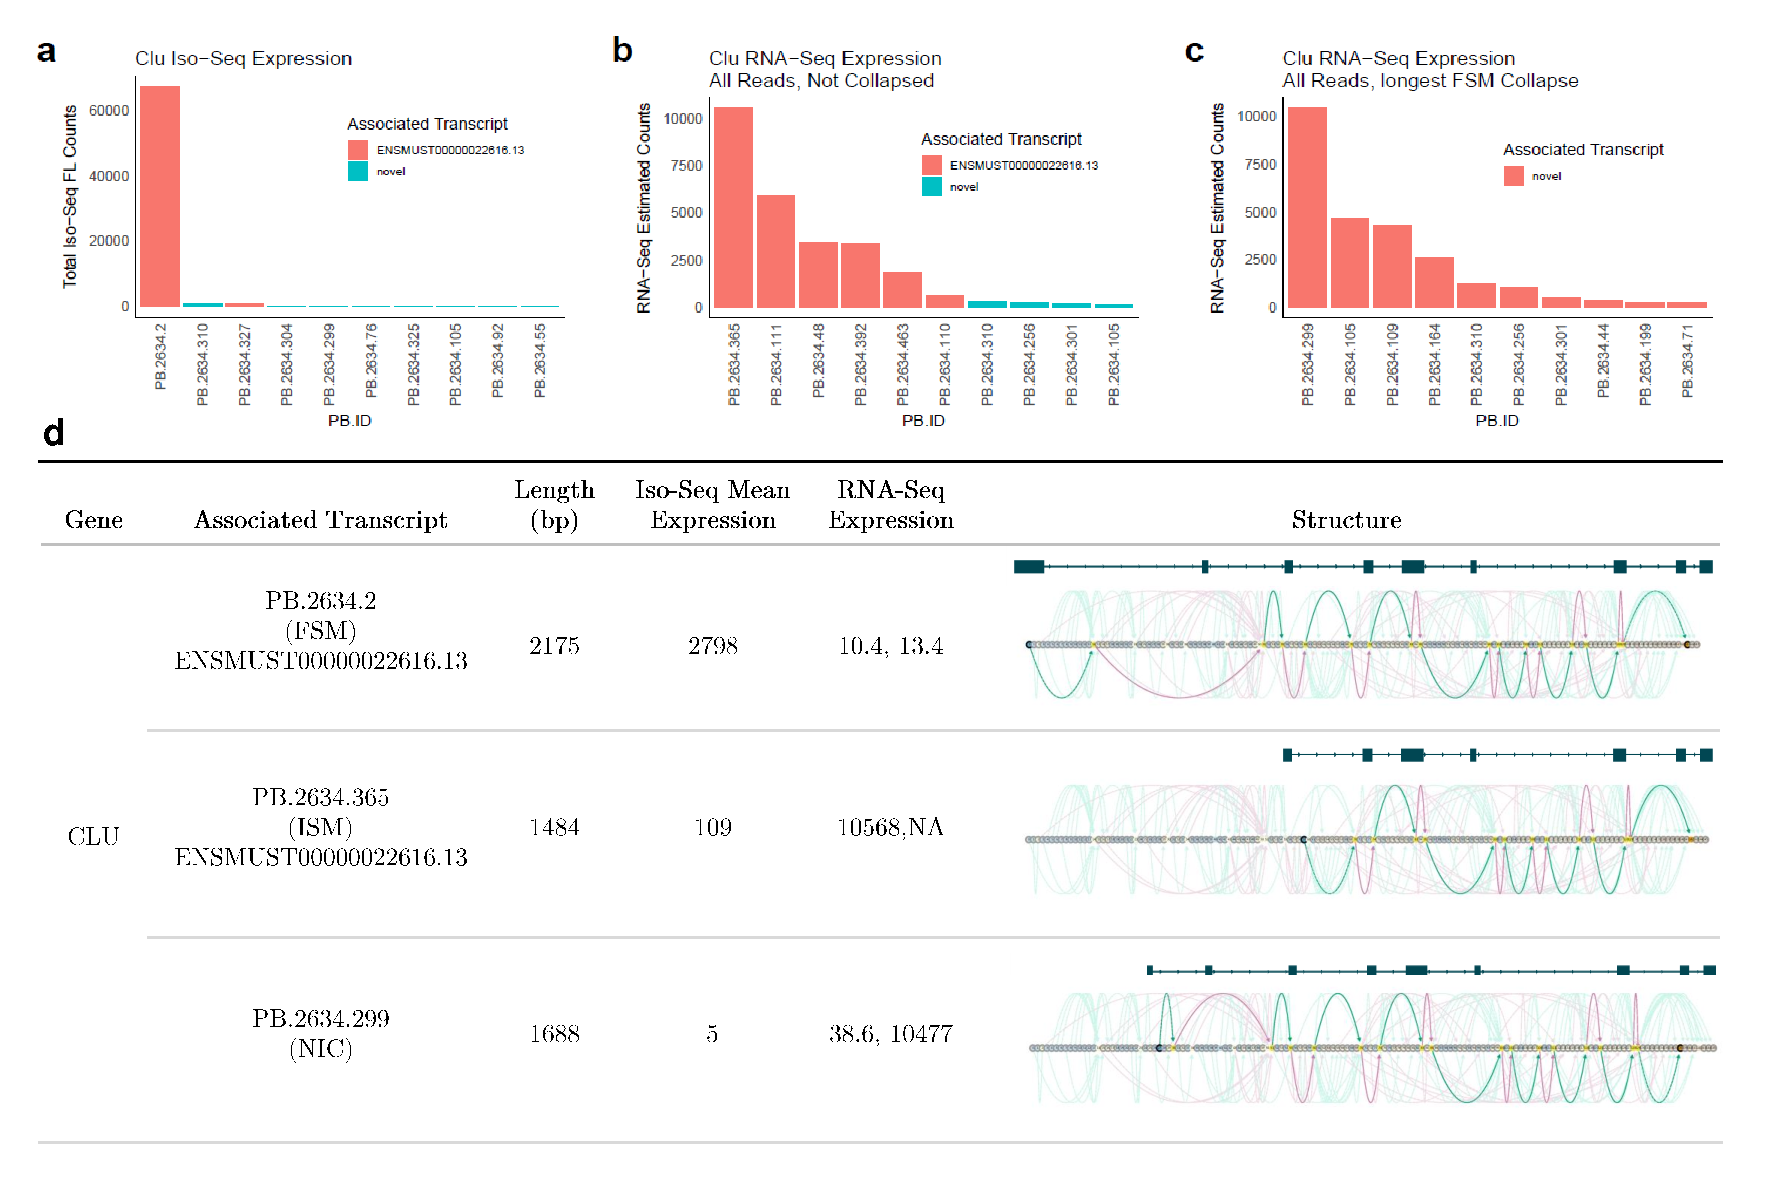
\includegraphics[page=1,trim={0cm 1cm 0cm 0cm},clip,scale = 0.8]{Figures/ProjectDevelopment_Figures_Landscape.pdf}
		\captionsetup{width=1.2\textwidth,singlelinecheck=off}
		\caption[RNA-Seq mis assignment of dominant isoform associated with \textit{Clu}]%
		{\textbf{RNA-Seq mis assigns \textit{Clu}'s novel isoform as most abundantly expressed}. Shown are the top 10 most abundantly expressed \textit{Clu} transcripts based on \textbf{A)} Iso-Seq full-length read counts from targeted transcriptome, \textbf{B)} RNA-Seq reads aligned to all reads in targeted transcriptome, with no further collapse of redundant FSM and ISM transcripts (Method 1 in \cref{tab:rnaseq_alignment_targeted}) and \textbf{C)} RNA-Seq reads aligned to all reads in targeted transcriptome with isoforms further collapsed to longest FSM (Method 2 in \cref{tab:rnaseq_alignment_targeted}). Of note, all other methods (3 - 6) generated a similar plot to figure c. \textbf{D)} Swan visualisations of most abundantly expressed isoforms according to respective methods. Iso-Seq mean expression refer to average full length read counts from targeted transcriptome. RNA-Seq mean expression refer to estimated counts from \textit{Kallisto} in Figures b and c. 
		}
		\label{fig:Clu_TargetedRNAseqAlignment}
	\end{figure}
	
	
	\begin{figure}[htp]
		\centering
		\includegraphics[page=2,trim={0cm 0cm 0cm 0cm},clip,scale = 0.8]{Figures/ProjectDevelopment_Figures_Landscape.pdf}
		\captionsetup{width=1.2\textwidth,singlelinecheck=off}
		\caption[RNA-Seq mis-assignment of dominant isoform associated with \textit{Bin1}]%
		{\textbf{RNA-Seq mis-assigns \textit{Bin1}'s novel isoform as most abundantly expressed}. Shown are the top 10 most abundantly expressed \textit{Bin1} transcripts based on \textbf{A)} Iso-Seq full-length read counts from targeted transcriptome, \textbf{B)} RNA-Seq reads aligned to all reads in targeted transcriptome, with no further collapse of redundant FSM and ISM transcripts (Method 1 in \cref{tab:rnaseq_alignment_targeted}) and \textbf{C)} RNA-Seq reads aligned to all reads in targeted transcriptome with isoforms further collapsed to longest FSM (Method 2 in \cref{tab:rnaseq_alignment_targeted}). Of note, all other methods (3 - 6) generated a similar plot to figure c. \textbf{D)} Swan visualisations of most abundantly expressed isoforms according to respective methods. Iso-Seq mean expression refer to average full length read counts from targeted transcriptome. RNA-Seq mean expression refer to estimated counts from \textit{Kallisto} in Figures b and c. 
		}
		\label{fig:Bin1_TargetedRNAseqAlignment}
	\end{figure}
\end{landscape}
\restoregeometry


%Alternative splicing events?

\boldheader{Mapt}
7 known isoforms detected (ENSMUST00000106992.9, ENSMUST00000100347.10, ENSMUST00000138384.7, ENSMUST00000106988.7, ENSMUST00000126820.1, ENSMUST00000132245.7, ENSMUST00000106993.9) with ENSMUST00000106992.9 the dominant isoform. 
56 novel isoforms detected (22 NIC and 34 NNC), 4 with intron retention and 6 predicted for NMD.  
RNA-Seq expression and Iso-Seq expression show very different profile due to RNA-Seq reads also from sequencing transgene human \textit{MAPT} - conversely any full-length transcript containing human \textit{MAPT} transgene would have been filtered out during Iso-Seq bioinformatics pipeline, thus Iso-Seq reads would only capture mouse \textit{MAPT} isoforms. Unable to use RNA-Seq reads due to sequencing of human transgene; No differential mouse \textit{MAPT} gene or transcript expression. 
Antisense transcript to MAPT also detected.
%Of note: 2 ISMs have have semi high expression counts and may be multimapped; apply a threshold to ensure that must have more than x number of exons from the known but caveats?
%humanMAPT decreases but progressive tau pathology?


\subsection{Alternative splicing in Target Genes}
\begin{itemize}
	\item Sorl1: intron retention and two were predicted for NMD (PB.8560.84 with a different polyA motif and PB.8560.39)
	\item Bin1: multiple intron retention events; 11 isoforms were characterised with intron retention, of which all but one was predicted for NMD. 9 additional isoforms were predicted for NMD. - higher level of intron retention in AD mice?
	\item Ptk2b: 6 isoforms with intron retention
\end{itemize}


\subsection{Isoform expression}
\begin{itemize}
	\item Detected many novel isoforms using Iso-Seq reads with lower expression
	\item Despite detecting many isoforms, some genes only have one dominant isoform which is typically the known (Sorl1, Tardbp, Clu, particularly in the case with APP with 118 isoforms detected)
	\item Some isoforms that appear to be all similarly expressed (Picalm)
	\item Very lowly expressed Trpa1 and Rhbdf2 with only one isoform and three isoforms detected respectively
\end{itemize}

\subsection{Differential transcript expression}

\begin{itemize}
	\item As would be expected, target transcriptome detected more isoforms per associated gene than whole transcriptome (with the exception of \textit{Ank1,Snca}) and lowly-expressed genes not otherwise detected in whole transcriptome, including \textit{Cd33},\textit{Rhbdf2}, \textit{Trpa1}
	\item Across all genes independent of sequencing approach, RNA-Seq expression of associated gene and isoform is significantly higher than corresponding Iso-Seq expression, reflecting of higher sequencing coverage and sample size 
	\item Except for \textit{Trem2}, differential gene and transcript expression was only identified in whole transcriptome when RNA-Seq was used as expression (rather than Iso-Seq)
	\item This observation was recapitulated in targeted transcriptome with \textit{Abca1} and \textit{Clu}
\end{itemize}

\begin{itemize}
	\item Abca1: RNA-Seq expression identified differential gene and isoform expression with increased expression of known isoform with progressive tau pathology. A smaller general trend is observed with Iso-Seq data alone but insignificant.
	\item Bin1 Differential transcript expression observed using Iso-Seq reads with increased expression of novel isoform (PB.3915.524, NIC, P = 3.66 x 10\textsuperscript{-5}, R-squared = 0.547), but this was not recapitulated with RNA-Seq reads.
	\item Tardby: 18 novel isoforms, the majority of which were characterised with intron retention (n = 14) and also predicted for NMD (n = 8) and 3 additional for NMD
	\item App: Differential transcript expression observed using Iso-Seq reads with increased expression of known isoform (ENSMUST00000227654.1, P = 1.75 x 10\textsuperscript{-8}, R-squared = 0.657), but this was not recapitulated with RNA-Seq reads
	\item Sorl1: Differential transcript expression observed using Iso-Seq reads with increased expression of known isoform (ENSMUST00000089250.8, P = 2.317 x 10\textsuperscript{-8}, R-squared = 0.634), but this was not recapitulated with RNA-Seq reads.
	\item Clu: Differential gene and isoform expression was detected using RNA-Seq reads as expression, with upregulated expression associated with progressive tau pathology. However, this increase expression was attributed to a novel isoform (G4103.43,PB.2634.299) rather than the known longer isoform
	\item Differential gene expression identified using both Iso-Seq and RNA-Seq reads as expression with TG showing increased gene expression across progressive tau pathology. Iso-Seq attributed this increase to the known isoform (PB.7333.28, ENSMUST00000173739.7), whereas RNA-Seq attributed this increase to the novel isoform (G11287.50)
	\item Cd33: Differential gene expression and isoform expression was observed using both Iso-Seq and RNA-Seq reads, driven by upregulated expression of the known isoform (PB.7476.2), which was also detected in the whole transcriptome. 
	\item Observed significant differential gene expression and transcript expression - increased gene expression associated with progressive tau pathology, which is attributed to the known isoform (ENSMUST00000024791.14).
\end{itemize}

\subsection{Differential transcript usage}

